% explanation.tex --- the paralever proofs, written out long-form.
%
% A companion to ~/papers/paper-paralever/main.tex.  It covers the same material
% as that paper's sections 3-7, in the same order, but written for a reader who
% knows none of it: every symbol is defined before use, every proof is given in
% full with its cases named, and each hard step is preceded by a worked example
% on concrete numbers.
%
% Compiles standalone:  pdflatex explanation.tex  (three passes for references)
%
% Deliberately NO Lean declaration names.  The \lean macro is defined as a
% no-op, so prose copied across from main.tex drops its [Lean: ...] tags
% silently instead of breaking.

\documentclass[11pt,a4paper]{article}

\usepackage[T1]{fontenc}
\usepackage[utf8]{inputenc}
\usepackage[margin=1in]{geometry}
\usepackage{amsmath,amssymb,amsthm}
\usepackage{mathtools}
\usepackage{listings}
\usepackage{xcolor}
\usepackage{hyperref}
\usepackage{booktabs}
\usepackage{tikz}
\usetikzlibrary{arrows.meta,positioning,fit}
\usepackage{enumitem}

\hypersetup{colorlinks=true,linkcolor=black,citecolor=black,urlcolor=blue}
\setlength{\emergencystretch}{3em}

\theoremstyle{definition}
\newtheorem{definition}{Definition}
\theoremstyle{plain}
\newtheorem{theorem}[definition]{Theorem}
\newtheorem{lemma}[definition]{Lemma}
\newtheorem{corollary}[definition]{Corollary}
\newtheorem{proposition}[definition]{Proposition}
\newtheorem{claim}[definition]{Claim}
\theoremstyle{remark}
\newtheorem{remark}[definition]{Remark}
\newtheorem{example}[definition]{Example}

% Scratch work before a proof, and the moral after it.  Both are part of the
% argument here, not decoration: the first says how the proof was found, the
% second says what it taught.
\newenvironment{scratch}{\par\medskip\noindent\textit{Scratch work.}\ \ignorespaces}{\par\medskip}
\newenvironment{moral}{\par\medskip\noindent\textit{The moral.}\ \ignorespaces}{\par\medskip}

% A no-op, on purpose.  See the header.
\newcommand{\lean}[1]{}

\newcommand{\PM}{\texttt{ParM}}
\newcommand{\st}{\sigma}
\newcommand{\Loc}{\mathsf{Loc}}
\newcommand{\Val}{\mathsf{Val}}
\newcommand{\State}{\mathsf{State}}
\newcommand{\reads}[1]{R(#1)}
\newcommand{\writes}[1]{W(#1)}
\newcommand{\acc}{\mathsf{accesses}}
\newcommand{\runSeq}{\mathsf{runSeq}}
\newcommand{\wf}{\mathsf{WellFormed}}
\newcommand{\Indep}{\mathsf{Indep}}
\newcommand{\work}{\mathsf{work}}
\newcommand{\spn}{\mathsf{time}}
\newcommand{\pstep}{\mathsf{pstep}}
\newcommand{\Reaches}{\mathsf{Reaches}}
\newcommand{\wrong}{\mathbf{wrong}}
\newcommand{\upd}[3]{#1[#2 \mapsto #3]}

% Lean listings, ASCII only: `->' for the arrow, `|->' for the map-to.  Keeping
% them ASCII means no `literate' table to go stale, and nothing silently
% vanishes from a listing.
\definecolor{leanKw}{HTML}{1D4ED8}
\definecolor{leanTy}{HTML}{0F766E}
\definecolor{leanCom}{HTML}{6B7280}
\lstdefinestyle{lean}{
  basicstyle=\ttfamily\footnotesize,
  sensitive=true,
  alsoletter={_},
  keywordstyle=\bfseries\color{leanKw},
  morekeywords={def,theorem,inductive,structure,where,match,with,fun,let,if,then,else},
  keywordstyle=[2]\color{leanTy},
  morekeywords=[2]{ParM,Childs,Results,Loc,Val,State,Prop,Type,Unit,Nat,Int,Bool,List,Option,
    Footprint,Conf,pure,read,write,par,nil,cons,some,none,run,wrong},
  commentstyle=\color{leanCom}\itshape,
  morecomment=[l]{--},
  columns=fullflexible,
  keepspaces=true,
  showstringspaces=false,
  xleftmargin=1.2em,
  aboveskip=0.6em,belowskip=0.6em,
}
\lstset{style=lean}

\title{Why a Parallel Program Equals Its Sequential Reading\\
       \large The paralever proofs, written out in full}
\author{}
\date{}

\begin{document}
\maketitle
\vspace{-3em}

\section*{How to read this}

This document proves one theorem: a parallel program whose branches do not interfere
produces exactly the same answer as the sequential program that runs those branches one
after another --- under \emph{every} possible interleaving, not just the ones we thought
to try.

It assumes nothing. Every symbol is defined before it is used, every proof is given with
its cases named and none of them waved away, and each difficult step is preceded by the
same step worked by hand on concrete numbers. Where a hypothesis is doing real work, we
also show what breaks when it is dropped.

It follows the sequence of the paper, section for section:

\begin{center}\small
\begin{tabular}{@{}lll@{}}
\toprule
\textbf{Here} & \textbf{Paper} & \textbf{Contents} \\
\midrule
\S\ref{sec:question}  & ---   & the question, and a pair of programs that answers it badly \\
\S\ref{sec:model}     & \S3   & programs as data; why they are trees; why induction is awkward \\
\S\ref{sec:indep}     & \S4   & what a program touches; independence; the machine \\
\S\ref{sec:lang}      & \S5   & the surface language and its decidable check \\
\S\ref{sec:canonical} & \S6   & the theorem, and the equivalence read off it \\
\S\ref{sec:cost}      & \S7   & cost: same work, fewer rounds \\
\S\ref{sec:recap}     & ---   & the whole argument in nine lines, and where it breaks \\
\bottomrule
\end{tabular}
\end{center}

\noindent A reader who wants the theorem as fast as possible can read
\S\ref{sec:question}--\S\ref{sec:indep}, skip \S\ref{sec:lang} entirely, and go straight to
\S\ref{sec:canonical}. Nothing in \S\ref{sec:canonical} depends on \S\ref{sec:lang}; the
dependency runs the other way.

\tableofcontents

\section{The question}\label{sec:question}

Here are two programs. The first says ``do these two jobs at the same time''. The second
says ``do the first job, then the second''.
\[
  \mathtt{A[5] := 1} \quad\|\quad \mathtt{A[8] := A[7]}
  \qquad\text{against}\qquad
  \mathtt{A[5] := 1};\ \mathtt{A[8] := A[7]}
\]

Do they leave the same memory behind? Your instinct says yes, and here your instinct is
right. But consider this pair, which differs in one character:
\[
  \mathtt{A[5] := 1} \quad\|\quad \mathtt{A[8] := A[5]}
  \qquad\text{against}\qquad
  \mathtt{A[5] := 1};\ \mathtt{A[8] := A[5]}
\]

Run the sequential version from an all-zeros memory. Cell $5$ becomes $1$; then cell $8$
copies cell $5$, so cell $8$ ends up holding $1$. Now run the parallel version and let the
right-hand job go first: it copies cell $5$ while cell $5$ is still $0$, so cell $8$ ends
up holding $0$.

So the answer to the question is ``sometimes''. Our job is to find the exact condition
under which the answer is \emph{always yes}, and then prove it --- not test it, prove it,
for every program, every starting memory, and every way a machine might interleave the
work. Everything that follows is the machinery needed to state that claim precisely enough
to be provable, and then the proof.

Two remarks on what we are \emph{not} doing, because both shape the development.

We are not proving the parallel program has no races and then hoping determinism follows.
It does not: \S\ref{sec:recap:break} exhibits a program whose every individual step is
race-free at the instant it happens, and which still has two terminating runs that
disagree. The hypothesis has to be stronger than race freedom, and \S\ref{sec:indep:wf} is
where it gets defined.

We are also not proving a one-sided statement of the form ``if the parallel program
terminates then its answer is correct''. That is what a soundness theorem usually gives,
and it is satisfied by a program with no terminating runs at all. What we prove is an
equality of outcome \emph{sets}, which rules that out; the extra direction costs us
\S\ref{sec:canonical:live}.

\section{Programs as data}\label{sec:model}

A theorem relating a parallel program to a sequential one needs two things. Both programs
must be objects the logic can quantify over --- so we can say ``for every program
$p$\ldots'' --- and parallel composition must \emph{mean} something the logic does not
already know. Those two requirements pin the representation down almost completely, and
this section says how.

\subsection{Memory}\label{sec:model:heap}

We need to say what memory is. The simplest thing that works:

\begin{definition}[Addresses, values, memory]\label{def:heap}
An address is a natural number, $\Loc \coloneqq \mathbb{N}$. A value is drawn from a small
universe $\Val$ of storable things --- integers, booleans, unit. A \emph{memory} (we will
also say \emph{heap}) is a total function from addresses to values:
$\State \coloneqq \Loc \to \Val$.
\end{definition}

So a memory $\st$ is a function. To ask what is in cell $7$ you write $\st\,7$. Three
features of this choice matter later, and it is worth saying now which.

\emph{It is total} --- defined at every address. There is no unallocated cell, no null, no
crash on a bad read: $\st\,999999$ is perfectly well defined and holds whatever is there.
We therefore never carry a definedness side condition, and ownership of memory is expressed
by \emph{footprints} (\S\ref{sec:indep:fp}) rather than by a heap's domain. Programs in the
surface language do declare buffers and end their lifetimes, but that happens in the
compiler and leaves no trace in the program that runs (\S\ref{sec:lang:mem}).

\emph{Addresses are numbers}, not an opaque type, so a question like ``is $i \cdot n + j$
inside the block $[b,\ b+\ell)$?'' is ordinary linear arithmetic and a machine can decide
it. Richer value types are encoded into $\Val$ through a type class, never by adding
constructors to Definition~\ref{def:heap}.

\emph{Updating it builds a new function.}

\begin{definition}[Update]\label{def:update}
For a memory $\st$, an address $l$ and a value $v$,
\[
  \upd{\st}{l}{v} \;\coloneqq\; \lambda k.\ \text{if } k = l \text{ then } v \text{ else } \st\,k .
\]
\end{definition}

That is, $\upd{\st}{l}{v}$ is ``the same as $\st$, except cell $l$ now holds $v$''. Two
consequences are immediate from Definition~\ref{def:update}, and we will use them
constantly:
\begin{align}
  \upd{\st}{l}{v}\,l &= v \label{eq:f1}\\
  \upd{\st}{l}{v}\,k &= \st\,k \qquad\text{whenever } k \neq l \label{eq:f2}
\end{align}

\begin{remark}\label{rem:f2}
Equation~\eqref{eq:f2} is the single load-bearing fact in this document. Everything below
is machinery for lifting it from \emph{one cell} to \emph{whole programs}: Lemma~\ref{lem:frame}
lifts it to one program, Lemma~\ref{lem:locality} to a program observed on two memories,
Lemma~\ref{lem:isolated} to two sibling branches, and Lemma~\ref{lem:stepcombined} to a
single step of an arbitrary interleaving. If you keep one thing in mind while reading, keep
this: a write to cell $l$ cannot be seen at cell $k$.
\end{remark}

\subsection{Programs}\label{sec:model:parm}

Now: what is a program? Here is the design choice everything rests on. \textbf{A program is
a piece of data} --- a finite tree --- not a Lean function.

Why? Because we want to ask questions like ``which cells does this program write?''. You
cannot ask that of an opaque function; you can ask it of a tree. And because if parallel
composition were a Lean function, Lean's own equational theory would already fix its
meaning, and there would be nothing left to prove (\S\ref{sec:model:task} makes that
concrete).

A fork has to hold several programs at once, and those programs need not return the same
type: one child might compute an \texttt{Int} while its sibling computes a \texttt{Bool}.
An ordinary $\texttt{List}\ (\PM\ \texttt{Int})$ cannot hold both, so the children of a fork
get a type of their own, indexed by the list of types they return.

\begin{definition}[Children of a fork]\label{def:childs}
\begin{lstlisting}
def Results : List Type -> Type
  | []      => Unit
  | a :: as => a * Results as

inductive Childs (Node : Type -> Type 1) : List Type -> Type 1 where
  | nil  : Childs Node []
  | cons : Node a -> Childs Node as -> Childs Node (a :: as)
\end{lstlisting}
\end{definition}

Read both at the index $[\,\texttt{Int},\ \texttt{Bool}\,]$. A value of
$\texttt{Childs ParM}\ [\,\texttt{Int},\ \texttt{Bool}\,]$ is built by \texttt{cons},
\texttt{cons}, \texttt{nil} and holds exactly two programs, a $\PM\ \texttt{Int}$ and a
$\PM\ \texttt{Bool}$; no other value of that type exists. Meanwhile
$\mathsf{Results}\ [\,\texttt{Int},\ \texttt{Bool}\,]$ unfolds to
$\texttt{Int} \times (\texttt{Bool} \times \texttt{Unit})$ --- one factor per child, with
the \texttt{Unit} left over from the empty case. The index is thus a static record of how
many children a fork has and what each returns, so the continuation can be handed a tuple
of exactly the right shape.

\begin{definition}[Programs]\label{def:parm}
\begin{lstlisting}
inductive ParM : Type -> Type 1 where
  | pure  : a -> ParM a
  | read  : Loc -> (Val -> ParM a) -> ParM a
  | write : Loc -> Val -> (Unit -> ParM a) -> ParM a
  | par   : Childs ParM as -> (Results as -> ParM b) -> ParM b
\end{lstlisting}
\end{definition}

In words, the four node shapes are:
\begin{center}\small
\begin{tabular}{@{}ll@{}}
\toprule
$\texttt{pure}\ a$         & stop; the answer is $a$ \\
$\texttt{read}\ l\ k$      & read cell $l$, then continue as $k$ applied to the value you got \\
$\texttt{write}\ l\ v\ k$  & write $v$ into cell $l$, then continue as $k$ applied to $()$ \\
$\texttt{par}\ cs\ k$      & run everything in $cs$ at the same time, then continue as $k$ applied to all their answers \\
\bottomrule
\end{tabular}
\end{center}

\paragraph{Continuations sit inside the constructors.}
The odd-looking part is $k$. In $\texttt{read}\ l\ k$, the thing $k$ is a \emph{function}:
it takes the value that was read and returns the rest of the program. It has to be a
function, because what happens next genuinely depends on what was read --- if cell $7$
holds $3$ you might go one way, and if it holds $4$, another. So $\texttt{read}$ does not
``return a value''; it stores the remainder of the program as a function of the value. This
is called the \emph{freer} presentation of a monad, and $k$ is the \emph{continuation}.

A program is therefore a finite tree whose root is always the next action to perform and
whose leaves are all $\texttt{pure}$.

\begin{example}\label{ex:twoprogs}
The two jobs from \S\ref{sec:question}, written out. ``Write $1$ into cell $5$'' is
\[
  p \;\coloneqq\; \texttt{write}\ 5\ 1\ (\lambda \_.\ \texttt{pure}\ ())
\]
and ``copy cell $7$ into cell $8$'' is
\[
  q \;\coloneqq\; \texttt{read}\ 7\ (\lambda v.\ \texttt{write}\ 8\ v\ (\lambda \_.\ \texttt{pure}\ ())) .
\]
As trees, growing downward:
\begin{center}
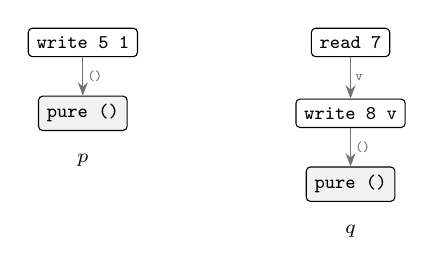
\begin{tikzpicture}[>=Stealth,
  n/.style  ={draw,rounded corners=1.5pt,inner sep=3pt,font=\scriptsize\ttfamily},
  lf/.style ={draw,rounded corners=1.5pt,inner sep=3pt,font=\scriptsize\ttfamily,fill=black!5},
  e/.style  ={draw,black!55,line width=0.4pt,->},
  lb/.style ={font=\tiny\ttfamily,inner sep=1.5pt,text=black!60}]
\node[n]  (p1) at (0,0)     {write 5 1};
\node[lf] (p2) at (0,-0.90) {pure ()};
\draw[e] (p1) -- node[lb,right] {()} (p2);
\node[font=\scriptsize] at (0,-1.5) {$p$};

\node[n]  (q1) at (3.4,0)     {read 7};
\node[n]  (q2) at (3.4,-0.90) {write 8 v};
\node[lf] (q3) at (3.4,-1.80) {pure ()};
\draw[e] (q1) -- node[lb,right] {v} (q2);
\draw[e] (q2) -- node[lb,right] {()} (q3);
\node[font=\scriptsize] at (3.4,-2.4) {$q$};
\end{tikzpicture}
\end{center}
We will carry $p$ and $q$ through the whole document.
\end{example}

\paragraph{Sequential composition is not a constructor.}
$\texttt{bind}\ p\ f$ walks the tree of $p$ and replaces every leaf $\texttt{pure}\ a$ with
the tree $f\,a$ (Figure~\ref{fig:graft}):
\[
\begin{array}{r@{\ }l}
  \texttt{bind}\ (\texttt{pure}\ a)\ f &= f\,a \\
  \texttt{bind}\ (\texttt{read}\ l\ k)\ f &= \texttt{read}\ l\ (\lambda v.\ \texttt{bind}\ (k\,v)\ f) \\
  \texttt{bind}\ (\texttt{write}\ l\ v\ k)\ f &= \texttt{write}\ l\ v\ (\lambda u.\ \texttt{bind}\ (k\,u)\ f) \\
  \texttt{bind}\ (\texttt{par}\ cs\ k)\ f &= \texttt{par}\ cs\ (\lambda vs.\ \texttt{bind}\ (k\,vs)\ f)
\end{array}
\]

Because the composite is an actual tree rather than a node recording that two trees were
composed, the monad laws are equalities \emph{of trees} and need no quotient. Left identity
$\texttt{bind}\ (\texttt{pure}\ a)\ f = f\,a$ is one unfolding of the definition. Right
identity and associativity take one induction each. Had \texttt{bind} been a constructor,
$\texttt{bind}\ (\texttt{bind}\ p\ f)\ g$ and
$\texttt{bind}\ p\ (\lambda a.\ \texttt{bind}\ (f\,a)\ g)$ would be two distinct trees that
we would have to identify by hand.

The same property removes evaluation contexts from the operational semantics of
\S\ref{sec:indep:step}: a small-step rule normally has to locate the redex somewhere inside
the term, and here it is always at the root.

\begin{figure}[htb]
\centering
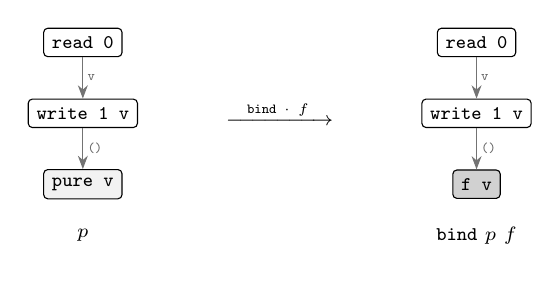
\begin{tikzpicture}[>=Stealth,
  n/.style  ={draw,rounded corners=1.5pt,inner sep=3pt,font=\scriptsize\ttfamily},
  lf/.style ={draw,rounded corners=1.5pt,inner sep=3pt,font=\scriptsize\ttfamily,fill=black!5},
  gr/.style ={draw,rounded corners=1.5pt,inner sep=3pt,font=\scriptsize\ttfamily,fill=black!18},
  e/.style  ={draw,black!55,line width=0.4pt,->},
  lb/.style ={font=\tiny\ttfamily,inner sep=1.5pt,text=black!60}]

\node[n]  (a1) at (0,0)     {read 0};
\node[n]  (a2) at (0,-0.90) {write 1 v};
\node[lf] (a3) at (0,-1.80) {pure v};
\draw[e] (a1) -- node[lb,right] {v} (a2);
\draw[e] (a2) -- node[lb,right] {()} (a3);
\node[font=\scriptsize] at (0,-2.45) {$p$};

\node[font=\scriptsize] at (2.5,-0.90) {$\xrightarrow{\ \ \texttt{bind}\ \cdot\ f\ \ }$};

\node[n]  (b1) at (5.0,0)     {read 0};
\node[n]  (b2) at (5.0,-0.90) {write 1 v};
\node[gr] (b3) at (5.0,-1.80) {f v};
\draw[e] (b1) -- node[lb,right] {v} (b2);
\draw[e] (b2) -- node[lb,right] {()} (b3);
\node[font=\scriptsize] at (5.0,-2.45) {$\texttt{bind}\ p\ f$};
\end{tikzpicture}
\caption{$p = \texttt{read}\ 0\ (\lambda v.\ \texttt{write}\ 1\ v\ (\lambda\_.\ \texttt{pure}\ v))$,
drawn as a tree. Each node stores the rest of the program as a function of what its own
effect returns, and each edge is labelled with the value passed on. $\texttt{bind}\ p\ f$
grafts $f$ onto the \texttt{pure} leaf and changes nothing else.}\label{fig:graft}
\end{figure}

\paragraph{The fork is $N$-ary and heterogeneous.}
A $\texttt{par}$ node holds one spine of $n$ children and one continuation receiving all $n$
results together. Binary parallelism is the case $n = 2$: it is not a second constructor,
and an $n$-child fork is not a tower of nested binary forks. Every theorem below is proved
at one fork with $n$ children. Two consequences recur: the race check at a fork compares all
$\binom{n}{2}$ pairs at once rather than spreading them over nesting levels, and a round of
the cost semantics (\S\ref{sec:cost}) advances all $n$ children together.

\paragraph{Every program terminates.}
$\PM$ is an \emph{inductive} type, so each of its values is a \emph{finite} tree and a
non-terminating loop cannot be written down at all. Lean 4 has no coinductive types, so this
is a boundary of the approach rather than an unfinished feature. Every example below is
structurally recursive or fuel-bounded with the fuel proved sufficient. This restriction is
not a nuisance we tolerate; it is what licenses Definition~\ref{def:runseq} to be a
\emph{function}, and Definition~\ref{def:runseq} is the whole proof strategy.

\begin{definition}[The two sides of the theorem]\label{def:combinators}
Write $\Pi[\,p\ q\,]$ for $\texttt{cons}\ p\ (\texttt{cons}\ q\ \texttt{nil})$. Then
\[
\begin{array}{r@{\ }l}
  \mathsf{parPair}\ p\ q &\coloneqq\ \texttt{par}\ \Pi[\,p\ q\,]\ (\lambda r.\ \texttt{pure}\ (r.1, r.2.1)) \\[2pt]
  \mathsf{seqPair}\ p\ q &\coloneqq\ \texttt{bind}\ p\ (\lambda a.\ \texttt{bind}\ q\ (\lambda b.\ \texttt{pure}\ (a,b))) \\[4pt]
  \mathsf{parAll}\ ps &\coloneqq\ \texttt{par}\ (\mathsf{childsOf}\ ps)\ (\lambda x.\ \texttt{pure}\ (\mathsf{resultsToList}\ ps\ x)) \\[2pt]
  \mathsf{seqAll}\ [\,] &\coloneqq\ \texttt{pure}\ [\,] \\
  \mathsf{seqAll}\ (p :: ps) &\coloneqq\ \texttt{bind}\ (\mathsf{seqPair}\ p\ (\mathsf{seqAll}\ ps))\ (\lambda r.\ \texttt{pure}\ (r.1 :: r.2))
\end{array}
\]
\end{definition}

Here $\mathsf{childsOf}$ turns a $\texttt{List}\ (\PM\ \alpha)$ into the spine
$\texttt{Childs ParM}\ [\alpha,\dots,\alpha]$ at the index repeating $\alpha$ once per
element, and $\mathsf{resultsToList}$ is its inverse on results, flattening the nested pairs
of $\mathsf{Results}$ back into a list. They are what let a homogeneous list be forked even
though $\texttt{par}$ is heterogeneous.

Note the asymmetry, because it is the shape of the theorem. $\mathsf{parAll}\ ps$ on a list
of $n$ programs is \emph{one} $\texttt{par}$ node with $n$ children. $\mathsf{seqAll}\ ps$ is
built from $\texttt{bind}$ alone and contains \emph{no} $\texttt{par}$ node whatsoever. These
are the two sides the equivalence theorem compares, and $\mathsf{parPair}/\mathsf{seqPair}$
are their two-child instances.

\subsection{Induction over a nested inductive}\label{sec:model:induction}

Lean's \texttt{induction} tactic does not work on $\PM$:
\begin{quote}\small
\texttt{The `induction' tactic does not support the type `ParM' because it is a nested
inductive type}
\end{quote}
This is the largest tax the representation imposes. It is paid once, by proving two
eliminators that every later proof uses, and the reason the tactic gives up determines the
shape of those two --- so it is worth a paragraph.

\paragraph{What a motive is.}
To prove $\forall p,\ P\,p$ by induction you must first say what is being proved about an
arbitrary $p$, \emph{as a function of} $p$. That function --- here $P$, of type
$\PM\ \alpha \to \mathtt{Prop}$ --- is called the \emph{motive}. A recursor takes the motive
first, then asks for one case per constructor, each case free to assume the motive at every
smaller program, and returns the motive at the program it was handed. The
\texttt{induction} tactic is a wrapper: it recovers the motive from the goal by abstracting
the goal over the variable being inducted on, then applies the recursor.

\paragraph{Why recovering it from the goal is not enough here.}
$\PM$ is defined in terms of $\texttt{Childs ParM}$, so Lean generates a recursor that
proves two things at once and takes \emph{two} motives:
\begin{lstlisting}
ParM.rec : {motive_1 : (a : Type) -> ParM a -> Sort u} ->
           {motive_2 : (as : List Type) -> Childs ParM as -> Sort u} ->
           (four cases for ParM, then two for Childs) ->
           (p : ParM a) -> motive_1 a p
\end{lstlisting}
A goal $P\,p$ fixes $\mathit{motive}_1$ and says \emph{nothing at all} about
$\mathit{motive}_2$: it mentions a program and never mentions a spine of children, so there
is nothing for the tactic to abstract. Choosing $\mathit{motive}_2$ is therefore a genuine
decision, and two choices are useful.

\begin{proposition}[Induction principles]\label{prop:induction}
Let $\mathit{motive} : (\alpha : \mathtt{Type}) \to \PM\ \alpha \to \mathtt{Prop}$.
\begin{enumerate}[label=(\roman*),leftmargin=2.2em,itemsep=2pt]
\item \textbf{Single-motive induction} proves
$\forall \alpha\ (p : \PM\ \alpha),\ \mathit{motive}\ \alpha\ p$ from four cases, one per
constructor. Its $\texttt{par}$ case may assume the motive of the continuation at every
tuple of results, and the motive of every child, the latter packaged as
$\mathsf{All}\ \mathit{motive}\ cs$ --- an iterated conjunction defined by
$\mathsf{All}\ \mathit{motive}\ \texttt{nil} = \mathtt{True}$ and
$\mathsf{All}\ \mathit{motive}\ (\texttt{cons}\ p\ ps) =
 \mathit{motive}\ p \wedge \mathsf{All}\ \mathit{motive}\ ps$.
\item \textbf{Mutual induction} takes a second motive
$\mathit{motive}_2 : (\alpha s : \mathtt{List\ Type}) \to \texttt{Childs ParM}\ \alpha s \to \mathtt{Prop}$
of its own and proves the \emph{pair}
\[
  \bigl(\forall \alpha\ (p : \PM\ \alpha),\ \mathit{motive}_1\,\alpha\,p\bigr) \ \wedge\
  \bigl(\forall \alpha s\ (cs : \texttt{Childs ParM}\ \alpha s),\ \mathit{motive}_2\,\alpha s\,cs\bigr)
\]
from six cases: the four above, with the $\texttt{par}$ case now assuming
$\mathit{motive}_2\,\alpha s\,cs$, plus $\mathit{motive}_2$ of the empty spine, plus a
$\texttt{cons}$ case deriving $\mathit{motive}_2\,(\alpha :: \alpha s)$ from
$\mathit{motive}_1\,\alpha$ for the head and $\mathit{motive}_2\,\alpha s$ for the tail.
\end{enumerate}
\end{proposition}

\begin{proof}
Both pick $\mathit{motive}_2$ in the generated recursor and then discharge its two
$\texttt{Childs}$ cases themselves, so that what reaches the caller is only the four $\PM$
cases.

For (i), take $\mathit{motive}_2\ cs \coloneqq \mathsf{All}\ \mathit{motive}\ cs$. The
$\texttt{nil}$ case then asks for $\mathsf{All}\ \mathit{motive}\ \texttt{nil}$, which
unfolds to $\mathtt{True}$. The $\texttt{cons}$ case is handed $\mathit{motive}$ of the head
and $\mathsf{All}\ \mathit{motive}$ of the tail, and must produce
$\mathsf{All}\ \mathit{motive}\ (\texttt{cons}\ p\ ps)$, which unfolds to the conjunction of
exactly those two. Both obligations are immediate, and that is the whole content of the
choice: it makes the children's statement be the program's statement, repeated.

For (ii), pass $\mathit{motive}_2$ through unchanged; the recursor gives the first component
directly. The second component is a separate, ordinary induction on $cs$, which is legal
because $\texttt{Childs}$ is an \emph{unnested} inductive: its $\texttt{nil}$ case is the
hypothesis for the empty spine, and its $\texttt{cons}$ case applies the $\texttt{cons}$
hypothesis to the first component at the head and to the inductive hypothesis at the tail.
\end{proof}

\begin{moral}
Which eliminator a proof needs depends on whether the claim about a spine of children is the
\emph{same} claim as the one about a program. For $\texttt{bind}$ it is: $\texttt{bind}$
leaves a fork's children untouched and only extends its continuation, so (i) suffices. For
execution it is not: $\runSeq$ acts on a program while $\mathsf{runChilds}$ acts on a spine,
and they are different functions, so the children-level claim must be stated separately and
the two proved together by (ii).

Every proof in \S\ref{sec:indep} and \S\ref{sec:canonical} is of the second kind: each is
stated as a conjunction of a program-level and a children-level claim, and in each the
$\texttt{cons}$ case assumes the claim for the head child and for the rest of the spine and
concludes it for the whole spine. We call that case the \textbf{$2$-to-$N$ step} throughout.
It is the same argument every time, which is why the $N$-ary development is no longer than a
binary one would have been.
\end{moral}

\subsection{Why not Lean's \texttt{Task}}\label{sec:model:task}

Lean provides \texttt{Task} for genuine runtime parallelism, and it is tempting to state the
theorem about that. The attempt is not merely inconvenient; it is \emph{vacuous}.
\texttt{Task} is a one-field structure whose body is the value, so
\[
  (\texttt{Task.spawn}\ f).\texttt{get} \;=\; f\ ()
\]
holds by $\texttt{rfl}$ --- by unfolding definitions. The parallel program and the
sequential one are then \emph{the same term}, and any equivalence between them is an
identity with no content. The hypothesis could be deleted and the theorem would still hold.

The general principle: \textbf{the meaning of $\texttt{par}$ must be supplied by us, and must
be genuinely interleaving, or there is nothing to prove.} That rules out a shallow
embedding, where $\texttt{par}$ would be a Lean function and Lean's equational theory would
fix its meaning; it equally rules out treating a compiled runtime as the semantics. It does
\emph{not} require deep-embedding the whole language: binders, data types, arithmetic and
recursion are all inherited from Lean, and only the four constructs whose interleaving
behaviour is at issue get reified. \texttt{Task} remains the compilation \emph{target}, and
nothing is ever proved there.

\begin{moral}
Because a program is data, one tree can be read in many ways, and the development is
organised around exactly that: $\mathsf{step}$ is the operational semantics
(\S\ref{sec:indep:step}), $\runSeq$ the canonical run (\S\ref{sec:indep:runseq}), $\acc$ the
footprint (\S\ref{sec:indep:fp}), $\work$ and $\pstep$ the cost measures
(\S\ref{sec:cost}), and there is a compiler to \texttt{Task}. A shallow embedding gives you
only the first.
\end{moral}

\section{What a program touches, and the machine that runs it}\label{sec:indep}

This section defines the two sides of the main theorem: the \emph{hypothesis} you discharge
per program, and the \emph{relation} the conclusion is stated over. It closes with four
locality lemmas that connect them.

\subsection{The reference run}\label{sec:indep:runseq}

Here is the first interpreter, and it is deliberately boring. It takes a program and a
memory and returns the answer and the final memory. \textbf{It contains no parallelism at
all}: at a $\texttt{par}$ node it runs child $1$ to completion, then child $2$ from where
child $1$ stopped, then child $3$, and so on.

\begin{definition}[The canonical run]\label{def:runseq}
\[
\begin{array}{r@{\ }l}
  \runSeq\ (\texttt{pure}\ a)\ \st &= (a, \st) \\
  \runSeq\ (\texttt{read}\ l\ k)\ \st &= \runSeq\ (k\,(\st\,l))\ \st \\
  \runSeq\ (\texttt{write}\ l\ v\ k)\ \st &= \runSeq\ (k\,())\ \upd{\st}{l}{v} \\
  \runSeq\ (\texttt{par}\ cs\ k)\ \st &= \runSeq\ (k\,vs)\ \tau
    \qquad\text{where } (vs, \tau) = \mathsf{runChilds}\ cs\ \st
\end{array}
\]
and the children run strictly left to right, each from the memory the previous one left:
\[
\begin{array}{r@{\ }l}
  \mathsf{runChilds}\ [\,]\ \st &= ((), \st) \\
  \mathsf{runChilds}\ (p :: ps)\ \st &= ((a, ws), \tau_2)
    \quad\text{where } (a, \tau_1) = \runSeq\ p\ \st \text{ and } (ws, \tau_2) = \mathsf{runChilds}\ ps\ \tau_1
\end{array}
\]
\end{definition}

Why is this allowed to be a function rather than a relation? Because programs are finite
trees (\S\ref{sec:model:parm}), so the recursion always bottoms out: every case recurses
into a strictly smaller tree, or into a continuation applied to a value already in hand.
This is plain structural recursion, with no cleverness and no termination argument to
supply.

\begin{remark}[Why this is the whole strategy]\label{rem:strategy}
$\runSeq$ is the \emph{reference answer}. It is deterministic, total and computable. The
main theorem will say: the real parallel machine, under every schedule whatsoever, agrees
with $\runSeq$. We will never compare the parallel program to the sequential one directly.
We will show both of them equal this third thing.
\end{remark}

\begin{example}[The reference run, by hand]\label{ex:runseq}
Let $\st_0$ be the all-zeros memory, $\st_0\,l = 0$ for every $l$, and take $p$, $q$ from
Example~\ref{ex:twoprogs}. Running $p$:
\begin{align*}
  \runSeq\ (\texttt{write}\ 5\ 1\ (\lambda\_.\ \texttt{pure}\ ()))\ \st_0
    &= \runSeq\ (\texttt{pure}\ ())\ \upd{\st_0}{5}{1} && \text{(the \texttt{write} rule)} \\
    &= ((),\ \upd{\st_0}{5}{1}) && \text{(the \texttt{pure} rule)}
\end{align*}
Write $\st_1 \coloneqq \upd{\st_0}{5}{1}$. Running $q$ from $\st_1$:
\begin{align*}
  \runSeq\ (\texttt{read}\ 7\ (\lambda v.\ \texttt{write}\ 8\ v\ \cdots))\ \st_1
    &= \runSeq\ (\texttt{write}\ 8\ (\st_1\,7)\ \cdots)\ \st_1 && \text{(the \texttt{read} rule)}
\end{align*}
and what is $\st_1\,7$? By~\eqref{eq:f2}, since $7 \neq 5$, it is $\st_0\,7 = 0$. So the run
continues to $((),\ \upd{\st_1}{8}{0})$.

Now the fork. By Definition~\ref{def:runseq}, $\mathsf{runChilds}\ \Pi[\,p\ q\,]\ \st_0$ runs
$p$ from $\st_0$, reaching $\st_1$, then $q$ from $\st_1$, reaching $\upd{\st_1}{8}{0}$.
Hence
\[
  \runSeq\ (\mathsf{parPair}\ p\ q)\ \st_0 = \bigl(((),()),\ \upd{\upd{\st_0}{5}{1}}{8}{0}\bigr) .
\]
Cell $5$ holds $1$ and cell $8$ holds $0$. Keep that memory in mind; we will meet it again
in Example~\ref{ex:isolated} and \S\ref{sec:canonical:parseq}.
\end{example}

\subsection{Footprints}\label{sec:indep:fp}

To state the condition under which parallel equals sequential, we must talk about
\emph{which cells} a program touches. So: a second interpreter, walking the same tree,
collecting addresses instead of computing answers.

\begin{definition}[Footprints]\label{def:footprint}
A $\mathsf{Footprint}$ is a pair of lists of addresses, the cells read and the cells
written, written $f = (\reads{f}, \writes{f})$, with
\[
  f \cup g \coloneqq (\reads{f} \mathbin{+\!\!+} \reads{g},\ \writes{f} \mathbin{+\!\!+} \writes{g}),
  \qquad \mathsf{empty} \coloneqq ([\,],[\,]) .
\]
\end{definition}

Lists rather than finite sets, because every question we ask of a footprint is a membership
test or a disjointness test. Duplicates are therefore harmless, and a concrete footprint
stays computable. Union is associative with $\mathsf{empty}$ as a unit, so folding
footprints needs no bracketing convention.

\begin{definition}[The footprint of a program]\label{def:acc}
\[
\begin{array}{r@{\ }l}
  \acc\ (\texttt{pure}\ a)\ \st &= \mathsf{empty} \\
  \acc\ (\texttt{read}\ l\ k)\ \st &= ([l],[\,]) \cup \acc\ (k\,(\st\,l))\ \st \\
  \acc\ (\texttt{write}\ l\ v\ k)\ \st &= ([\,],[l]) \cup \acc\ (k\,())\ \upd{\st}{l}{v} \\
  \acc\ (\texttt{par}\ cs\ k)\ \st &= \mathsf{accChilds}\ cs\ \st \cup \acc\ (k\,vs)\ \tau
    \qquad (vs,\tau) = \mathsf{runChilds}\ cs\ \st \\[3pt]
  \mathsf{accChilds}\ [\,]\ \st &= \mathsf{empty} \\
  \mathsf{accChilds}\ (p :: ps)\ \st &= \acc\ p\ \st \cup \mathsf{accChilds}\ ps\ (\runSeq\ p\ \st).2
\end{array}
\]
\end{definition}

\paragraph{Why a footprint needs a memory argument.}
This confuses every reader once, so let us be careful. Look at the $\texttt{read}$ clause.
To see what happens \emph{after} the read we need $k$ applied to something, and $k$ is a
function expecting the value read --- so we must supply $\st\,l$. There is no way to look
past a $\texttt{read}$ without saying what it returned. \textbf{A program's footprint is a
function of the memory it starts in.} That is not a defect of the definition; it is forced
by continuations, and it is why $\acc$ is a fold over the same tree $\runSeq$ walks rather
than a syntactic function.

Concretely, $\texttt{read}\ 7\ (\lambda v.\ \texttt{write}\ v\ 1\ \cdots)$ writes to a cell
whose \emph{address} comes out of cell $7$. Change the starting memory and it writes
somewhere else. \S\ref{sec:lang:fp} is about recovering a syntactic bound anyway, at a
stated cost in precision.

\begin{example}[Footprints, by hand]\label{ex:acc}
Continuing Example~\ref{ex:runseq},
\begin{align*}
  \acc\ p\ \st_0 &= ([\,],[5]) \cup \acc\ (\texttt{pure}\ ())\ \st_1 = ([\,],[5]) \cup \mathsf{empty} = ([\,],[5]) \\
  \acc\ q\ \st_1 &= ([7],[\,]) \cup \bigl( ([\,],[8]) \cup \mathsf{empty} \bigr) = ([7],[8])
\end{align*}
So $p$ reads nothing and writes cell $5$; $q$ reads cell $7$ and writes cell $8$. Exactly
what one would say by eye --- the definition is doing the right thing.
\end{example}

\subsection{The staggered measurement}\label{sec:indep:stagger}

\begin{definition}[Per-child footprints]\label{def:childfootprints}
\begin{align*}
  \mathsf{childFootprints}\ [\,]\ \st &= [\,] \\
  \mathsf{childFootprints}\ (p :: ps)\ \st &= \acc\ p\ \st :: \mathsf{childFootprints}\ ps\ \tau_1,
    \qquad (\_,\tau_1) = \runSeq\ p\ \st
\end{align*}
\end{definition}

This keeps one footprint \emph{per child}, where $\mathsf{accChilds}$ merged them all into
one. The distinction matters: $\mathsf{accChilds}$ is what you want when a fork is treated as
a single unit, and $\mathsf{childFootprints}$ is what the all-pairs independence check ranges
over.

\begin{remark}[The crux of the entire theorem]\label{rem:stagger}
Look at \emph{where} each child is measured. Child $1$ is measured at $\st$. Child $2$ is
measured at $(\runSeq\ p\ \st).2$ --- the memory \textbf{after child $1$ has completely
finished}. Child $3$ after children $1$ and $2$ have finished. And so on.

\emph{But the real parallel machine will not run child $2$ at that memory.} It may run child
$2$ first, at $\st$. So we are about to define our hypothesis using one memory while the
machine uses a different one, and nothing written so far says the two agree.

This gap is the whole technical content of the theorem. It is closed, once, in
Lemma~\ref{lem:isolated}, and the one place it is \emph{used} is sub-case B of
Lemma~\ref{lem:stepcombined}. Every other case of every other proof is bookkeeping.
\end{remark}

For our running example,
\[
  \mathsf{childFootprints}\ \Pi[\,p\ q\,]\ \st_0 = [\ ([\,],[5]),\ ([7],[8])\ ],
\]
and the second entry was measured at $\st_1$, not at $\st_0$.

\subsection{Independence}\label{sec:indep:indep}

\begin{definition}[Bernstein independence]\label{def:indep}
$\Indep\ f_1\ f_2$ holds when all three of these sets are empty:
\[
  \text{(C1)}\ \ \writes{f_1} \cap \writes{f_2} = \emptyset, \qquad
  \text{(C2)}\ \ \writes{f_1} \cap \reads{f_2} = \emptyset, \qquad
  \text{(C3)}\ \ \writes{f_2} \cap \reads{f_1} = \emptyset .
\]
\end{definition}

Three clauses, and the reader must notice \emph{which one is missing}: there is no clause
$\reads{f_1} \cap \reads{f_2} = \emptyset$. Two computations may read the same cell as much
as they like, because reading changes nothing and nobody can tell who read first.

That omission is load-bearing rather than a convenience. Matrix multiplication computes each
output cell $C[i,j]$ in its own thread; the threads write disjoint cells, so (C1)--(C3)
hold, but every thread in row $i$ reads the whole of row $i$ of $A$. A criterion with a
fourth clause on reads would reject matrix multiplication, and with it most of the programs
anyone wants to parallelise. (A separation-logic $\ast$ is exactly such a criterion, which
is the subject of the paper's related-work section.)

\begin{example}[Independent, and not]\label{ex:indep}
For $p$ and $q$ of Example~\ref{ex:twoprogs}, with $f_1 = ([\,],[5])$ and $f_2 = ([7],[8])$:
\[
  \text{(C1) } \{5\} \cap \{8\} = \emptyset \ \checkmark \qquad
  \text{(C2) } \{5\} \cap \{7\} = \emptyset \ \checkmark \qquad
  \text{(C3) } \{8\} \cap \emptyset = \emptyset \ \checkmark
\]
so $\Indep\ f_1\ f_2$ holds.

Now replace $q$ by the broken sibling of \S\ref{sec:question},
$q' \coloneqq \texttt{read}\ 5\ (\lambda v.\ \texttt{write}\ 8\ v\ \cdots)$, which copies
cell $5$ instead of cell $7$. Then $\acc\ q'\ \st_1 = ([5],[8])$ and
\[
  \text{(C2) } \writes{f_1} \cap \reads{f_2} = \{5\} \cap \{5\} = \{5\} \neq \emptyset \ \times
\]
so independence fails. This is precisely the program whose two schedules disagreed. The
condition catches it, and clause (C2) is the one that does.
\end{example}

\begin{definition}[The $N$-ary obligation]\label{def:indepall}
$\mathsf{IndepAll}\ [\,] = \mathtt{True}$ and
$\mathsf{IndepAll}\ (f :: fs) = \bigl(\forall g \in fs,\ \Indep\ f\ g\bigr) \wedge \mathsf{IndepAll}\ fs$.
\end{definition}

Unfolded, this is pairwise independence of all $\binom{n}{2}$ pairs, stated flatly rather
than spread across nesting levels, and $\mathsf{IndepAll}\ [f_1,f_2]$ is just
$\Indep\ f_1\ f_2$.

\begin{proposition}[Everything here is decidable]\label{prop:decide}
There are Boolean functions $\mathsf{disjointB}$, $\mathsf{indepB}$, $\mathsf{indepAllB}$
with $\mathsf{indepB}\ f_1\ f_2 = \mathtt{true} \leftrightarrow \Indep\ f_1\ f_2$ and
$\mathsf{indepAllB}\ fs = \mathtt{true} \leftrightarrow \mathsf{IndepAll}\ fs$.
\end{proposition}

\begin{proof}
Take $\mathsf{disjointB}\ a\ b \coloneqq a.\mathsf{all}\ (\lambda l.\ \neg\,b.\mathsf{contains}\ l)$,
which decides disjointness of two lists because a universally quantified Boolean test over a
list is equivalent to its $\mathsf{all}$. Then $\mathsf{indepB}$ is the conjunction of three
such checks, matching Definition~\ref{def:indep} clause for clause, and
$\mathsf{indepAllB}$ follows by induction on the list.
\end{proof}

This is what makes the hypothesis cheap in practice: for a concrete program and memory the
whole obligation is discharged by evaluation, often by $\mathtt{rfl}$.

\subsection{Well-formedness: the hypothesis}\label{sec:indep:wf}

\begin{definition}[Well-formedness]\label{def:wf}
\[
\begin{array}{r@{\ }l}
  \wf\ (\texttt{pure}\ a)\ \st &= \mathtt{True} \\
  \wf\ (\texttt{read}\ l\ k)\ \st &= \wf\ (k\,(\st\,l))\ \st \\
  \wf\ (\texttt{write}\ l\ v\ k)\ \st &= \wf\ (k\,())\ \upd{\st}{l}{v} \\
  \wf\ (\texttt{par}\ cs\ k)\ \st &= \mathsf{IndepAll}\ (\mathsf{childFootprints}\ cs\ \st) \\
    &\phantom{{}={}} {}\wedge\ \mathsf{wfChilds}\ cs\ \st
      \ \wedge\ \wf\ (k\,vs)\ \tau \\[3pt]
  \mathsf{wfChilds}\ [\,]\ \st &= \mathtt{True} \\
  \mathsf{wfChilds}\ (p :: ps)\ \st &= \wf\ p\ \st \ \wedge\ \mathsf{wfChilds}\ ps\ \tau_1
\end{array}
\]
where $(vs,\tau) = \mathsf{runChilds}\ cs\ \st$ in the fork clause and
$(\_,\tau_1) = \runSeq\ p\ \st$ in the children clause.
\end{definition}

In words: \textbf{walk the whole tree along the canonical run, and at every $\texttt{par}$
node you meet, check that all pairs of its children are independent at the memory that node
sees.} The three conjuncts at a fork each do a job: the children do not interfere with each
other; each child is itself well-formed, since it may contain forks of its own; and
whatever follows the join is well-formed too.

\paragraph{Why not just check the outermost fork?}
Because a child can race \emph{with itself} while the two children stay disjoint from each
other. Take
\[
  \texttt{par}\ \Pi[\ \underbrace{\texttt{par}\ \Pi[\,\texttt{write}\ 3\ \ \texttt{write}\ 3\,]}_{\text{child }1}
                 \ \ \underbrace{\texttt{write}\ 99}_{\text{child }2}\ ] .
\]
Child $1$'s total footprint is $\{3\}$ and child $2$'s is $\{99\}$: disjoint, so an
outermost-only check passes. But child $1$ is a race. Hence the recursion in
Definition~\ref{def:wf}. This is the only obligation discharged per program; everything in
\S\ref{sec:canonical} is proved once and for all.

\begin{example}\label{ex:wf}
$\wf\ (\mathsf{parPair}\ p\ q)\ \st_0$ unfolds to three conjuncts:
$\mathsf{IndepAll}\ [([\,],[5]), ([7],[8])]$, which holds by Example~\ref{ex:indep};
$\wf\ p\ \st_0 \wedge \wf\ q\ \st_1 \wedge \mathtt{True}$, all trivially true since neither
contains a $\texttt{par}$ node; and $\wf$ of a $\texttt{pure}$ leaf, also trivial. So the
running example is well-formed.
\end{example}

\subsection{The real machine}\label{sec:indep:step}

Everything so far was reference material. \textbf{Now we define the machine that is actually
allowed to interleave}, and it is this machine the theorem is about.

First we need to detect races: two threads about to touch one cell with at least one write.

\begin{definition}[Labels and conflict]\label{def:label}
A $\mathsf{Label}$ is $\texttt{read}\ l$ or $\texttt{write}\ l$. Two labels \emph{conflict}
when they name the same address and at least one is a write. Values are irrelevant to races
and are not recorded.
\end{definition}

\begin{definition}[Ready actions and the race test]\label{def:racing}
$\mathsf{nextAccs}\ p$ collects the actions $p$ could perform \emph{right now}:
\[
  \mathsf{nextAccs}\ (\texttt{pure}\ a) = [\,], \quad
  \mathsf{nextAccs}\ (\texttt{read}\ l\ k) = [\texttt{read}\ l], \quad
  \mathsf{nextAccs}\ (\texttt{write}\ l\ v\ k) = [\texttt{write}\ l],
\]
and $\mathsf{nextAccs}\ (\texttt{par}\ cs\ k)$ is all the children's ready actions
flattened, so a deeply nested program contributes every one of its live heads and no pair is
missed. $\mathsf{nextAccsChilds}\ cs$ keeps one list \emph{per} child. Then
$\mathsf{racing}\ as\ bs$ holds when some action in $as$ conflicts with some action in $bs$,
and $\mathsf{racingAll}$ holds when some \emph{two distinct} children's lists race.
\end{definition}

Keeping one list per child, rather than one flat list, is what lets $\mathsf{racingAll}$
compare pairs of children while ignoring a child's conflicts with itself. One thread about
to write cell $3$ and later write it again is not a race; two threads both about to write
cell $3$ are.

\begin{definition}[All children finished]\label{def:allpure}
$\mathsf{allPure}\ cs$ is $\mathsf{some}\ vs$ when every child is a $\texttt{pure}$ leaf,
collecting their values into the tuple the continuation expects, and $\mathsf{none}$ as soon
as one child still has work left.
\end{definition}

\begin{definition}[Configurations and one step]\label{def:step}
A configuration is $\texttt{run}\ p\ \st$ or $\wrong$. The step function returns the
\emph{list} of configurations we could move to:
\[
\begin{array}{r@{\ }l}
  \mathsf{step}\ (\texttt{pure}\ a)\ \st &= [\,] \\
  \mathsf{step}\ (\texttt{read}\ l\ k)\ \st &= [\ \texttt{run}\ (k\,(\st\,l))\ \st\ ] \\
  \mathsf{step}\ (\texttt{write}\ l\ v\ k)\ \st &= [\ \texttt{run}\ (k\,())\ \upd{\st}{l}{v}\ ] \\
  \mathsf{step}\ (\texttt{par}\ cs\ k)\ \st &=
    \begin{cases}
      [\ \wrong\ ] & \text{if } \mathsf{racingAll}\ (\mathsf{nextAccsChilds}\ cs) \\
      [\ \texttt{run}\ (k\,vs)\ \st\ ] & \text{else if } \mathsf{allPure}\ cs = \mathsf{some}\ vs \\
      \text{one successor per ready child} & \text{otherwise, via } \mathsf{stepChilds}
    \end{cases}
\end{array}
\]
Here $\mathsf{stepChilds}\ cs\ \st$ advances \emph{any one} child and rebuilds the spine
around it; it is type-preserving, and a child aborting is inherited by the whole fork.
Finally $\mathsf{stepC}$ lifts $\mathsf{step}$ to configurations, with
$\mathsf{stepC}\ \wrong = [\,]$.
\end{definition}

\paragraph{The list \emph{is} the nondeterminism.}
This is the key idea of the semantics, and it is why no schedulers or thread identifiers
appear anywhere. A $\texttt{par}$ node with three children that can all move returns a list
of \emph{three} configurations, and each is a different choice the machine could make. All
possible interleavings are exactly all the paths you can trace through these lists, and
nothing outside the list counts as a schedule.

\paragraph{The \texttt{par} case is a trichotomy.}
Exactly one of the three branches fires (Figure~\ref{fig:trichotomy}). The second and third
cannot both apply, because if every child is a finished leaf then no child can move:

\begin{proposition}[Join and step are exclusive]\label{prop:joinexcl}
If $\mathsf{allPure}\ cs$ is defined then $\mathsf{stepChilds}\ cs\ \st = [\,]$.
\end{proposition}

\begin{proof}
Induction on $cs$. The $\texttt{nil}$ case is immediate. The $\texttt{cons}$ case: for
$\mathsf{allPure}$ to be defined the head must be $\texttt{pure}\ a$, whose $\mathsf{step}$
is the empty list, and the tail is handled by the induction hypothesis; a concatenation of
two empty lists is empty.
\end{proof}

\begin{figure}[htb]
\centering
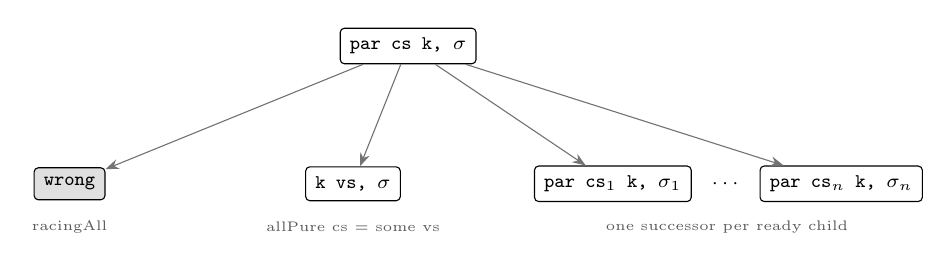
\begin{tikzpicture}[>=Stealth, font=\small,
  c/.style  ={draw,rounded corners=1.5pt,inner sep=3.5pt,font=\scriptsize\ttfamily},
  w/.style  ={draw,rounded corners=1.5pt,inner sep=3.5pt,font=\scriptsize\ttfamily,fill=black!12},
  e/.style  ={draw,black!55,line width=0.4pt,->},
  g/.style  ={font=\tiny,inner sep=1.5pt,text=black!65,align=center}]

\node[c] (top) at (0,0) {par cs k, $\sigma$};
\node[w] (wr)  at (-4.3,-1.75) {wrong};
\node[c] (jn)  at (-0.7,-1.75) {k vs, $\sigma$};
\node[c] (m1)  at ( 2.6,-1.75) {par cs$_1$ k, $\sigma_1$};
\node[c] (m2)  at ( 5.5,-1.75) {par cs$_n$ k, $\sigma_n$};
\node[font=\scriptsize] at (4.05,-1.75) {$\cdots$};

\draw[e] (top) -- (wr); \draw[e] (top) -- (jn);
\draw[e] (top) -- (m1); \draw[e] (top) -- (m2);
\node[g] at (-4.3,-2.30) {racingAll};
\node[g] at (-0.7,-2.30) {allPure cs $=$ some vs};
\node[g] at (4.05,-2.30) {one successor per ready child};
\end{tikzpicture}
\caption{The \texttt{par} case of $\mathsf{step}$. The three branches are tried in this
order and are mutually exclusive (Proposition~\ref{prop:joinexcl}). Only the third produces
more than one successor, and that is the only place a schedule is ever
chosen.}\label{fig:trichotomy}
\end{figure}

\paragraph{$\wrong$ is a black hole.}
It has no successors, so it is terminal and absorbing. A racy program is not assigned a
behaviour that we then have to reason about --- it falls off the edge of the world and is
\emph{excluded}. This is why we never argue about whether memory operations are atomic: a
racy program has no outcomes at all, so the question never arises. The race test moreover
runs at \emph{every} step, not only at the start, so a run that never reaches $\wrong$ is
race-free at every instant.

\begin{example}[A step with two successors]\label{ex:step}
Take $\mathsf{parPair}\ p\ q$ at $\st_0$. We have
$\mathsf{nextAccs}\ p = [\texttt{write}\ 5]$ and
$\mathsf{nextAccs}\ q = [\texttt{read}\ 7]$. Different cells, so no conflict, so
$\mathsf{racingAll}$ is false --- branch one does not fire. Is $\mathsf{allPure}$ defined?
No: $p$ is a $\texttt{write}$ node, not a leaf --- branch two does not fire. So branch three
gives a list of \emph{two} configurations:
\[
  \bigl[\ \texttt{run}\ (\texttt{par}\ \Pi[\,\texttt{pure}\ ()\ \ q\,]\ k)\ \upd{\st_0}{5}{1},
  \quad \texttt{run}\ (\texttt{par}\ \Pi[\,p\ \ \texttt{write}\ 8\ 0\,]\ k)\ \st_0\ \bigr]
\]
--- one in which $p$ went first, one in which $q$ went first. Those are the two schedules,
and the theorem must hold down both of them, and down every branch of every branch.

Change $q$ to $q'$ (which reads cell $5$) and the same call returns the single successor
$[\wrong]$: now $\texttt{write}\ 5$ and $\texttt{read}\ 5$ conflict.
\end{example}

\begin{definition}[Reachability]\label{def:reaches}
$\Reaches$ is the reflexive--transitive closure of $\mathsf{stepC}$, generated by
$\Reaches\ c\ c$ and, from $\Reaches\ c\ c'$ together with $c'' \in \mathsf{stepC}\ c'$,
$\Reaches\ c\ c''$. We write $\mathsf{Safe}\ c$ for $\neg\,\Reaches\ c\ \wrong$. The
children-level closure $\mathsf{ReachesChilds}$ is defined the same way from
$\mathsf{stepChilds}$, relating one pair $(cs,\st)$ to another with nobody having aborted.
\end{definition}

$\Reaches$ is the object every statement about ``all interleavings'' is really about.
\textbf{We never quantify over schedules explicitly}: a schedule \emph{is} a path through
the closure, so the closure does the quantification for us. $\mathsf{ReachesChilds}$
replaces the left-branch and right-branch lemmas a binary development would need --- with
$n$ children there is no left and right, only ``some child moved''.

\begin{proposition}[Basic properties of $\Reaches$]\label{prop:reachesbasic}
$\Reaches$ is transitive; a configuration with no successors reaches only itself; and if
$\mathsf{stepC}\ c = [c_0]$ then $\Reaches\ c\ c'$ implies $c' = c$ or
$\Reaches\ c_0\ c'$. $\mathsf{ReachesChilds}$ is transitive.
\end{proposition}

\begin{proof}
Each by induction on the closure. The third is the deterministic-step case analysis, used
for $\texttt{read}$ and $\texttt{write}$, whose successor lists are singletons: either the
run stopped where it was, or its first move went to the unique successor.
\end{proof}

\subsection{What we want to prove}\label{sec:indep:goal}

\begin{definition}[Outcome equivalence]\label{def:parseqeq}
Programs $p$ and $q$ are \emph{outcome-equivalent from $\st$}, written
$p \mathrel{\|\!\equiv} q$, when for every answer $r$ and every final memory $\st'$,
\[
  \Reaches\ \langle p, \st\rangle\ \langle \texttt{pure}\ r, \st'\rangle
  \ \longleftrightarrow\
  \Reaches\ \langle q, \st\rangle\ \langle \texttt{pure}\ r, \st'\rangle .
\]
\end{definition}

That is: exactly the same set of possible finishing states. The goal of
\S\ref{sec:canonical} is
\[
  \wf\ (\mathsf{parPair}\ p\ q)\ \st
  \ \Longrightarrow\
  \mathsf{parPair}\ p\ q \mathrel{\|\!\equiv} \mathsf{seqPair}\ p\ q \text{ from } \st .
\]

\subsection{Locality: four lemmas}\label{sec:indep:locality}

A computation cannot observe what it does not touch. The four lemmas below make that precise
in four steps --- a program does not change cells outside its writes
(Lemma~\ref{lem:frame}); it computes the same thing on two memories that agree wherever it
looks (Lemma~\ref{lem:locality}); so an independent neighbour's run is invisible to it
(Lemma~\ref{lem:isolated}); and therefore the two can never race
(Lemma~\ref{lem:norace}). All four are about footprints and the canonical run, with no
mention of interleaving anywhere. \S\ref{sec:canonical} uses them in exactly that order.

\subsubsection{Frame}

\begin{lemma}[Frame]\label{lem:frame}
If $l \notin \writes{\acc\ p\ \st}$ then $(\runSeq\ p\ \st).2\ l = \st\ l$, and likewise for
$\mathsf{runChilds}$ against $\mathsf{accChilds}$.
\end{lemma}

\begin{scratch}
The claim is ``a program leaves alone what it does not write''. For a single
$\texttt{write}\ l'$ node this is exactly~\eqref{eq:f2}. So the proof should be an induction
whose only non-trivial case is $\texttt{write}$, and in that case the hypothesis should hand
us $l \neq l'$. Let us check that it does.
\end{scratch}

\begin{proof}
By mutual induction on $p$ (Proposition~\ref{prop:induction}(ii)). Six cases.

\emph{Case $\texttt{pure}\ a$.} Here $\runSeq\ (\texttt{pure}\ a)\ \st = (a,\st)$, so the
final memory \emph{is} $\st$ and the claim reads $\st\ l = \st\ l$.

\emph{Case $\texttt{read}\ l'\ k$.} By Definition~\ref{def:acc},
$\acc\ (\texttt{read}\ l'\ k)\ \st = ([l'],[\,]) \cup \acc\ (k\,(\st\,l'))\ \st$. Taking
writes of both sides, the first summand contributes nothing, so
$\writes{\acc\ (\texttt{read}\ l'\ k)\ \st} = \writes{\acc\ (k\,(\st\,l'))\ \st}$. Hence our
hypothesis is literally the continuation's hypothesis. Since
$\runSeq\ (\texttt{read}\ l'\ k)\ \st = \runSeq\ (k\,(\st\,l'))\ \st$, the conclusion is
literally the continuation's conclusion, and the induction hypothesis at $k\,(\st\,l')$ and
$\st$ finishes the case.

\emph{Case $\texttt{write}\ l'\ v\ k$.} Now
$\writes{\acc\ (\texttt{write}\ l'\ v\ k)\ \st} = [l'] \mathbin{+\!\!+} \writes{\acc\ (k\,())\ \upd{\st}{l'}{v}}$,
and the hypothesis says $l$ is in neither part. From the first part, $l \neq l'$. From the
second, the induction hypothesis applies to $k\,()$ at the updated memory, giving
$(\runSeq\ (k\,())\ \upd{\st}{l'}{v}).2\ l = \upd{\st}{l'}{v}\ l$. Since $l \neq l'$,
equation~\eqref{eq:f2} rewrites the right-hand side to $\st\ l$. Chaining these with
$\runSeq\ (\texttt{write}\ l'\ v\ k)\ \st = \runSeq\ (k\,())\ \upd{\st}{l'}{v}$ gives the
claim. \textbf{This case is where~\eqref{eq:f2} is spent; everything else is plumbing.}

\emph{Case $\texttt{par}\ cs\ k$.} Writing $(vs,\tau) = \mathsf{runChilds}\ cs\ \st$, we have
$\writes{\acc\ (\texttt{par}\ cs\ k)\ \st} = \writes{\mathsf{accChilds}\ cs\ \st} \mathbin{+\!\!+} \writes{\acc\ (k\,vs)\ \tau}$,
so $l$ lies outside both. The children's conclusion gives $\tau\ l = \st\ l$; the
continuation's induction hypothesis gives
$(\runSeq\ (k\,vs)\ \tau).2\ l = \tau\ l$. Composing the two equalities gives the claim.

\emph{Children, empty spine.} $\mathsf{runChilds}\ [\,]\ \st = ((),\st)$, so the claim is
$\st\ l = \st\ l$.

\emph{Children, the $2$-to-$N$ step.} From
$\mathsf{accChilds}\ (p :: ps)\ \st = \acc\ p\ \st \cup \mathsf{accChilds}\ ps\ (\runSeq\ p\ \st).2$
we get that $l$ is outside the head's writes and outside the tail's writes. By the head's
induction hypothesis, $(\runSeq\ p\ \st).2\ l = \st\ l$: the head left $l$ alone, so the
tail starts from a memory already agreeing with $\st$ at $l$. By the tail's induction
hypothesis at that memory, the tail leaves $l$ alone too. Composing gives the claim.
\end{proof}

\begin{moral}
Lemma~\ref{lem:frame} is equation~\eqref{eq:f2} lifted from one cell-write to an arbitrary
program tree. Each case either does not touch memory or touches it once and
invokes~\eqref{eq:f2}.
\end{moral}

\subsubsection{Locality}

\begin{definition}\label{def:fdisjoint}
$\mathsf{FDisjoint}\ F\ f \coloneqq \bigl(F \cap \reads{f} = \emptyset\bigr) \wedge
\bigl(F \cap \writes{f} = \emptyset\bigr)$.
\end{definition}

Reads and writes are required disjoint from $F$ \emph{separately} rather than as one
condition on their concatenation, because $\cup$ puts all the reads together and then all
the writes, and a combined condition does not project through a nested union.

\begin{lemma}[Locality]\label{lem:locality}
Suppose
\begin{align}
  &\mathsf{FDisjoint}\ F\ (\acc\ p\ \st) && \text{($p$ does not touch $F$)} \label{eq:h1}\\
  &\st\ l = \st'\ l \text{ for every } l \notin F && \text{(the memories agree outside $F$)} \label{eq:h2}
\end{align}
Then all three of the following hold:
\[
  \text{(i) } \acc\ p\ \st = \acc\ p\ \st', \qquad
  \text{(ii) } (\runSeq\ p\ \st).1 = (\runSeq\ p\ \st').1,
\]
\[
  \text{(iii) } (\runSeq\ p\ \st).2\ l = (\runSeq\ p\ \st').2\ l \text{ for every } l \notin F,
\]
and likewise at the children level.
\end{lemma}

\begin{scratch}
One might hope to prove (ii) alone, since the answer is what we care about. It cannot be
done. To get through a $\texttt{read}$ node we must know the continuation is the \emph{same
program} on both sides, which needs the read to return the same value, which needs
$l' \notin F$ --- fine. But to get through the node \emph{after} it we must know the two
memories \emph{still} agree outside $F$, which is (iii); and to apply
hypothesis~\eqref{eq:h1} to that continuation we must know its footprint matches, which is
(i). Each conclusion is the fuel for the others. So we carry all three.
\end{scratch}

\begin{proof}
By mutual induction on $p$, carrying (i), (ii) and (iii) simultaneously.

\emph{Case $\texttt{pure}\ a$.} Both footprints are $\mathsf{empty}$, giving (i). Both runs
return $a$, giving (ii). The final memories \emph{are} $\st$ and $\st'$, which agree outside
$F$ by~\eqref{eq:h2}, giving (iii).

\emph{Case $\texttt{read}\ l'\ k$.} The address $l'$ is a read of this program, and
hypothesis~\eqref{eq:h1} says $F \cap \reads{\cdot} = \emptyset$, so
\[
  l' \notin F, \qquad\text{hence by~\eqref{eq:h2}}\qquad \st\ l' = \st'\ l' \eqqcolon v .
\]
\textbf{This is the heart of the lemma}: the read returns the same value on both sides, so
the continuation is literally the same program $k\,v$ in both runs and the two executions
cannot diverge. Hypothesis~\eqref{eq:h1} restricted to the second summand of the union gives
$\mathsf{FDisjoint}\ F\ (\acc\ (k\,v)\ \st)$, so the induction hypothesis applies to $k\,v$
at $\st$ and $\st'$. Conclusions (ii) and (iii) transfer unchanged, because
$\runSeq\ (\texttt{read}\ l'\ k)\ \st = \runSeq\ (k\,v)\ \st$ and likewise for $\st'$; and
(i) holds because both footprints are $([l'],[\,])$ unioned with the same thing.

\emph{Case $\texttt{write}\ l'\ v\ k$.} Hypothesis~\eqref{eq:h1}, write half, gives
$l' \notin F$. The continuation runs at the updated memories $\upd{\st}{l'}{v}$ and
$\upd{\st'}{l'}{v}$, and we must check these still agree outside $F$ --- it is not
automatic. Take any $m \notin F$. If $m = l'$, both memories give $v$ by~\eqref{eq:f1}. If
$m \neq l'$, both reduce to $\st\ m$ and $\st'\ m$ by~\eqref{eq:f2}, which agree
by~\eqref{eq:h2}. So~\eqref{eq:h2} is re-established at the updated memories,
and~\eqref{eq:h1} holds for the continuation. Apply the induction hypothesis; (i), (ii),
(iii) follow as before.

\emph{Case $\texttt{par}\ cs\ k$.} Write $(vs,\tau) = \mathsf{runChilds}\ cs\ \st$ and
$(vs',\tau') = \mathsf{runChilds}\ cs\ \st'$. Hypothesis~\eqref{eq:h1} applied to the union
$\mathsf{accChilds}\ cs\ \st \cup \acc\ (k\,vs)\ \tau$ gives $\mathsf{FDisjoint}\ F$ of both
summands. The children's statement then gives
$\mathsf{accChilds}\ cs\ \st = \mathsf{accChilds}\ cs\ \st'$, $vs = vs'$, and agreement of
$\tau$ with $\tau'$ outside $F$. Because $vs = vs'$, the continuation is the \emph{same
program} $k\,vs$ on both sides; its footprint is disjoint from $F$ and the two memories it
starts from agree outside $F$, so the induction hypothesis applies and delivers (i), (ii),
(iii).

\emph{Children, empty spine.} Footprints are $\mathsf{empty}$; answers are both $()$;
memories are $\st$ and $\st'$, agreeing outside $F$ by~\eqref{eq:h2}.

\emph{Children, the $2$-to-$N$ step.} From
$\mathsf{accChilds}\ (p :: ps)\ \st = \acc\ p\ \st \cup \mathsf{accChilds}\ ps\ (\runSeq\ p\ \st).2$
and~\eqref{eq:h1}, both summands are disjoint from $F$. Apply the induction hypothesis to the
head: same footprint, same answer, and the two post-memories agree outside $F$. Those
post-memories are exactly where the tail starts, so~\eqref{eq:h2} is re-established for the
tail, and~\eqref{eq:h1} for the tail is the second summand. Apply the induction hypothesis to
the tail and compose.
\end{proof}

\begin{moral}
Locality says a program's behaviour depends only on the cells in its own footprint. It is
the formal content of ``what you do not look at cannot affect you'', and it is the workhorse:
Lemmas~\ref{lem:isolated} and~\ref{lem:wflocality} are both instances of it, and
Lemma~\ref{lem:stepcombined} calls it twice.
\end{moral}

\subsubsection{Isolation}

Now we cash in, and close the gap of Remark~\ref{rem:stagger}.

\begin{lemma}[Isolation]\label{lem:isolated}
If $\Indep\ (\acc\ p\ \st)\ (\acc\ q\ (\runSeq\ p\ \st).2)$ then
\[
  \acc\ q\ (\runSeq\ p\ \st).2 = \acc\ q\ \st
  \qquad\text{and}\qquad
  (\runSeq\ q\ (\runSeq\ p\ \st).2).1 = (\runSeq\ q\ \st).1 .
\]
In words: \textbf{$q$ cannot tell whether $p$ has already run.}
\end{lemma}

\begin{scratch}
We want Lemma~\ref{lem:locality} with the two memories being $\st$ and $(\runSeq\ p\ \st).2$.
Lemma~\ref{lem:locality} needs a set $F$ such that $q$ does not touch $F$ and the two
memories agree outside $F$. Which set could possibly work? The only cells where the two
memories \emph{can} differ are the cells $p$ wrote. So take $F$ to be exactly that set and
check the two hypotheses against it. That is the entire proof.
\end{scratch}

\begin{proof}
Put $F \coloneqq \writes{\acc\ p\ \st}$, and write $f_1 \coloneqq \acc\ p\ \st$,
$f_2 \coloneqq \acc\ q\ (\runSeq\ p\ \st).2$.

\emph{Hypothesis~\eqref{eq:h1}, that $q$ does not touch $F$.} Unfolding
$\mathsf{FDisjoint}\ F\ f_2$ by Definition~\ref{def:fdisjoint}, we need two things:
\[
  F \cap \reads{f_2} = \emptyset \ \text{ i.e. } \ \writes{f_1} \cap \reads{f_2} = \emptyset,
  \qquad
  F \cap \writes{f_2} = \emptyset \ \text{ i.e. } \ \writes{f_1} \cap \writes{f_2} = \emptyset .
\]
These are clauses (C2) and (C1) of Definition~\ref{def:indep}, verbatim. Nothing to do.

\emph{Hypothesis~\eqref{eq:h2}, that the two memories agree outside $F$.} We need
$(\runSeq\ p\ \st).2\ l = \st\ l$ for every $l \notin F$. Since $F$ is precisely
$\writes{\acc\ p\ \st}$, this says ``$p$ leaves alone every cell it does not write'' --- which
is Lemma~\ref{lem:frame}, exactly.

Both hypotheses hold, so Lemma~\ref{lem:locality} applies to the program $q$ with the two
memories $(\runSeq\ p\ \st).2$ and $\st$. Its conclusions (i) and (ii) are the two claims.
\end{proof}

\begin{remark}\label{rem:c3}
We used clauses (C1) and (C2) and never touched (C3). Clause (C3), namely
$\writes{f_2} \cap \reads{f_1} = \emptyset$, is what the \emph{opposite} order of the pair
needs --- it is $q$ not disturbing $p$. Definition~\ref{def:indep} is symmetric because both
orders come up.
\end{remark}

\begin{example}[The gap, closed, on numbers]\label{ex:isolated}
With $p$, $q$, $\st_0$, $\st_1$ as in Example~\ref{ex:runseq}:
\[
  \acc\ q\ \st_1 = ([7],[8]) \qquad\text{and}\qquad \acc\ q\ \st_0 = ([7],[8]) .
\]
Equal --- and the reason is that when $q$ reads cell $7$ it gets $\st_1\,7$ in the first case
and $\st_0\,7$ in the second, and $\st_1\,7 = \st_0\,7$ precisely because
$7 \notin \writes{\acc\ p\ \st_0} = \{5\}$, which is clause (C2).

Now substitute the broken $q'$, which reads cell $5$. The footprints still match,
$([5],[8])$ either way, but the \emph{answers} do not: $q'$ writes $1$ into cell $8$ when
measured after $p$ and $0$ when measured before. Lemma~\ref{lem:isolated}'s conclusion
fails --- and it must, because its hypothesis fails:
$\writes{f_1} \cap \reads{f_2} = \{5\} \neq \emptyset$.
\end{example}

\begin{moral}
An independent branch really is computed in isolation: its footprint and its result do not
depend on whether the other branch has run. This is the content that separation logic
expresses as a splitting $\st_1 \ast \st_2$ of the heap --- obtained here without splitting
anything, and without a condition on shared reads.
\end{moral}

\subsubsection{No race, and locality of the obligation}

\begin{lemma}[Ready actions lie inside footprints]\label{lem:nextaccs}
Every label in $\mathsf{nextAccs}\ p$ has its address in $\writes{\acc\ p\ \st}$ if it is a
write and in $\reads{\acc\ p\ \st}$ if it is a read; likewise for
$\mathsf{nextAccsChilds}$ against $\mathsf{accChilds}$.
\end{lemma}

\begin{proof}
Mutual induction on $p$. For $\texttt{pure}$, $\mathsf{nextAccs}$ is empty and there is
nothing to check. For $\texttt{read}\ l\ k$, the single ready label is $\texttt{read}\ l$
and Definition~\ref{def:acc} puts $l$ in the reads; $\texttt{write}$ is symmetric. For a
fork, the ready labels are exactly the children's labels flattened, and $\acc$ contains
$\mathsf{accChilds}\ cs\ \st$ as a summand, which by the children's induction hypothesis
contains every child's ready address --- and a union only adds. The $2$-to-$N$ step: a ready
label belongs to the head or to one of the rest, and either way the union keeps it.
\end{proof}

\begin{lemma}[Independence excludes a race]\label{lem:norace}
If $\Indep\ (\acc\ P\ \st)\ (\acc\ Q\ \st)$ then
$\mathsf{racing}\ (\mathsf{nextAccs}\ P)\ (\mathsf{nextAccs}\ Q)$ is false. Consequently, if
$\mathsf{IndepAll}\ (\mathsf{childFootprints}\ cs\ \st)$ then
$\mathsf{racingAll}\ (\mathsf{nextAccsChilds}\ cs)$ is false.
\end{lemma}

\begin{scratch}
The claim is negative --- ``no race'' --- which is the standard signal for proof by
contradiction. So suppose there \emph{is} a conflicting pair and find which Bernstein clause
it violates.
\end{scratch}

\begin{proof}
Suppose $\mathsf{racing}\ (\mathsf{nextAccs}\ P)\ (\mathsf{nextAccs}\ Q)$ is true. By
Definition~\ref{def:racing} there are labels $a \in \mathsf{nextAccs}\ P$ and
$b \in \mathsf{nextAccs}\ Q$ that conflict, so by Definition~\ref{def:label} they name one
address $l$ and at least one is a write. Three cases, and by Lemma~\ref{lem:nextaccs} each
puts $l$ in a particular component of each side's footprint.
\begin{itemize}[leftmargin=1.6em,itemsep=1pt]
\item \emph{Both writes.} Then $l \in \writes{f_1} \cap \writes{f_2}$, contradicting (C1).
\item \emph{$a$ a write, $b$ a read.} Then $l \in \writes{f_1} \cap \reads{f_2}$, contradicting (C2).
\item \emph{$a$ a read, $b$ a write.} Then $l \in \writes{f_2} \cap \reads{f_1}$, contradicting (C3).
\end{itemize}
Every case contradicts a hypothesis, so no such pair exists.

For the $N$-ary consequence, induct on the children. The head cannot race any later child:
$\mathsf{IndepAll}$'s first conjunct gives independence of the head's footprint from each
later child's, hence --- by a union argument --- from their combined footprint, to which the
first part applies. The later children cannot race each other by the induction hypothesis.
This is the $2$-to-$N$ step for the race check.
\end{proof}

\begin{remark}
Lemma~\ref{lem:isolated} used two of Bernstein's clauses; Lemma~\ref{lem:norace} uses all
three. Between them the definition is used exactly, with nothing left over --- which is one
reason to believe Definition~\ref{def:indep} has the right number of clauses.
\end{remark}

\begin{lemma}[Locality of the obligation]\label{lem:wflocality}
$\wf$ and $\mathsf{childFootprints}$ are invariant under changing the memory off a
footprint-disjoint set $F$.
\end{lemma}

\begin{proof}
Mutual induction on the program, using Lemma~\ref{lem:locality} at each node to transport
the footprints the obligation is stated about. There is no new idea here; the lemma exists
because Lemma~\ref{lem:stepcombined} needs to move a hypothesis, not just a value, from one
memory to another.
\end{proof}

\section{The surface language}\label{sec:lang}

Everything so far has been about $\PM$, which is a \emph{type} of programs rather than a
language anyone writes. Its effect nodes carry Lean functions as continuations, and two
consequences follow for anything built on top. A $\PM$ term cannot be printed past its first
$\texttt{read}$, because what comes after a read \emph{is} a function of the value read; and
its footprint has to be obtained by simulating it against a memory
(Definition~\ref{def:acc}), because the addresses a continuation will touch are not visible
in the term. Both are tolerable when you assemble programs by hand out of combinators.
Neither survives contact with a compiler, which delivers instructions rather than closures.

$\texttt{ParProg}$ is the same programs with their computations as \emph{data}. It is a
first-order inductive type --- $\texttt{load}$ and $\texttt{store}$ for memory,
$\texttt{set}$ for register arithmetic, $\texttt{seq}$, $\texttt{par}$ over a list of
threads, $\texttt{label}$ for a named region, $\texttt{ifElse}$, and
$\texttt{loadAt}/\texttt{storeAt}$ for an address computed at run time --- together with two
interpretations into $\PM$: $\mathsf{execPar}$, which sends $\texttt{par}$ to the $\PM$
$\texttt{par}$ constructor, and $\mathsf{execSeq}$, which sends it to the corresponding
chain of binds.

No new semantics is introduced and no axiom is added. Every theorem in this section ends in
a statement about $\PM$ and is discharged by \S\ref{sec:canonical}. What the layer
contributes is that the three things you actually want --- printing the program, knowing its
footprint, and discharging its obligation --- become \emph{computations} instead of proofs.

Two structural facts about the language are worth stating, because the independence
obligation depends on them. The only parallel form is a block of threads, and it is
fork--join: threads are spawned together and joined together, with no construct letting one
wait on, signal, or lock against another. And registers are thread-private --- a
$\texttt{par}$ node hands each thread a copy of the register file and discards what the
threads leave in it. That is why a thread cannot return a value (it writes one), and it is
why the obligation is about memory alone.

\subsection{Memory is declared, not allocated}\label{sec:lang:mem}

An address is a number, and a program of any size needs those numbers to come from somewhere
other than the author's head. A \emph{layout} is where they come from. A declaration carries
a name, a shape and initial contents and \emph{no address}; the allocator places each buffer
where the previous one ended; and a subscript is resolved against the shape, row-major, so
$\mathtt{A}[i,j]$ is the literal $\mathit{base}_A + i\cdot c + j$ --- an ordinary constant by
the time \S\ref{sec:lang:fp} folds it. Nothing about $\PM$ or \S\ref{sec:canonical} knows
this layer exists.

What it buys is one hypothesis, discharged once instead of once per pair of arrays.

\begin{proposition}[Placement is disjoint]\label{prop:alloc}
Buffers placed consecutively from any start address are pairwise non-overlapping: of any two,
one ends no later than the other begins.
\end{proposition}

A declaration can also end. $\mathtt{free}\ A$ does two things and nothing else: the name
leaves scope, so a later mention of $A$ fails to compile; and when $A$ is the most recent
buffer placed, its cells go back to the cursor, so the next declaration is placed on them.
Freeing out of order leaves the hole, since the cursor only moves back from the top. Nothing
is zeroed and no location goes away --- a buffer declared on a freed range begins holding
what the previous occupant left. This is an arena, not a heap, and the fact to want about it
is not Proposition~\ref{prop:alloc}, which reuse falsifies on purpose, but this one:

\begin{proposition}[Live buffers are disjoint]\label{prop:arena}
In the layout produced by any list of declarations and frees, two buffers that are live at
the same time share no location.
\end{proposition}

\begin{proof}
Carry two invariants along the declaration list: every live buffer's cells lie below the
cursor, and no cell belongs to two live buffers. A declaration places a buffer at the cursor
and advances it, so the new buffer lies below the new cursor and, by the first invariant,
overlaps no existing live buffer. A free is where the two invariants meet: lowering the
cursor could strand a live buffer above it only if that buffer lay inside the range just
freed, which the second invariant has already excluded. Disjointness is stated over
\emph{cells}, which makes a zero-size buffer vacuously disjoint from everything.
\end{proof}

\paragraph{Why Definition~\ref{def:heap} is unaffected.}
Both forms are \emph{erased}. Neither emits a $\texttt{ParProg}$ node, so
$\mathtt{buf}\ A[2];\ A[0] \coloneqq 1;\ \mathtt{free}\ A$ compiles to
$\mathtt{[0]} \coloneqq 1$ on the nose. The placement happens in the compiler, before there
is a program to run: $\State$ is still $\Loc \to \Val$, still total, and still has no
operation that creates or destroys a location --- which is why ``no allocation'' remains the
right description of the semantics while the language in front of it declares and reclaims
memory. What a set of declarations decides is which addresses the program names and what the
initial memory is, and every theorem from \S\ref{sec:canonical} on is parametric in the
memory. So a different layout changes the numbers in an example and never an obligation.

\paragraph{Why there is no run-time version.}
Admitting $\mathtt{alloc}$ and $\mathtt{free}$ as \emph{statements} would cost
Theorem~\ref{thm:parseq} twice over. An allocator has to choose an address; two schedules
choose differently, so the final memories differ and an equality of memories is false for
reasons that have nothing to do with races. A run-time $\mathtt{free}$ is worse: Bernstein's
conditions are about reads and writes of locations, so two threads freeing one block, or one
freeing while another reads it, is an error that three empty intersections cannot see, and
$\Indep$ would have to be re-derived rather than reused. Compile-time placement avoids both
by leaving no trace in the program.

\subsection{The footprint is computed, not proved}\label{sec:lang:fp}

$\mathsf{footprintOf}$ reads a footprint off the syntax by a fold. The two interesting
clauses are the ones where an address is not a literal:
\begin{lstlisting}
def footprintOf : ParProg -> Footprint
  | .load _ l      => ([l], [])        | .store l _     => ([], [l])
  | .seq a b       => union (footprintOf a) (footprintOf b)
  | .par ss        => footprintsOf ss  | .label _ s     => footprintOf s
  | .loadAt _ a _  => (a.cells, [])    -- index unknown: bound by the whole array
  | .storeAt a _ _ => ([], a.cells)
  | .ifElse _ t e  => union (footprintOf t) (footprintOf e)
\end{lstlisting}
It costs nothing to evaluate, and it is related to the real footprint by one proposition.

\begin{proposition}[The syntactic footprint bounds the real one]\label{prop:langfp}
For every $s : \texttt{ParProg}$, register file $\rho$ and memory $\st$,
\[
  \acc\ (\mathsf{execPar}\ s\ \rho)\ \st \;\sqsubseteq\; \mathsf{footprintOf}\ s ,
\]
where $f \sqsubseteq g$ means containment of reads in reads and writes in writes. If moreover
$s$ contains no $\texttt{loadAt}$, $\texttt{storeAt}$ or $\texttt{ifElse}$, the containment
is an equality.
\end{proposition}

\begin{proof}
Induction on $s$ using the mutual eliminator of \S\ref{sec:model:induction}. The literal
cases are equalities by Definition~\ref{def:acc}. For $\texttt{ifElse}$ the real footprint is
that of whichever arm runs, and each arm is contained in the union of the two. For
$\texttt{loadAt}$ and $\texttt{storeAt}$ the index wraps on the array's length by
construction, so the real access lies inside the array's cells, which is the stated bound.
\end{proof}

Containment is all the obligation needs, and that is a fact about Bernstein rather than a
convenience.

\begin{lemma}[Independence is antitone]\label{lem:antitone}
If $f' \sqsubseteq f$ and $g' \sqsubseteq g$ and $\Indep\ f\ g$, then $\Indep\ f'\ g'$.
\end{lemma}

\begin{proof}
All three clauses of Definition~\ref{def:indep} assert that an intersection is empty, and
shrinking either operand of an intersection cannot make it non-empty. Each clause transfers
directly.
\end{proof}

\begin{remark}
Lemma~\ref{lem:antitone} is why over-approximating a footprint is sound: widening a read set
can never manufacture a conflict, because there is \emph{no clause} on
$\reads{p} \cap \reads{q}$ to violate. Under $\ast$-disjointness the same move would be
unsound, since there enlarging a footprint enlarges the claimed ownership. The missing fourth
clause of Definition~\ref{def:indep} thus pays for itself a second time.
\end{remark}

\subsection{The obligation is decided}\label{sec:lang:wfb}

$\mathsf{wfB}$ is Definition~\ref{def:wf} read off the syntax: Bernstein at every
$\texttt{par}$ node, between every pair of its threads.
\begin{lstlisting}
def wfB : ParProg -> Bool
  | .load _ _ | .store _ _ | .set _ _ => true
  | .seq a b                          => wfB a && wfB b
  | .par ss       => indepAllB (threadFootprints ss) && wfAllB ss
  | .label _ s    => wfB s
  | .ifElse _ t e => wfB t && wfB e   -- either branch may run
\end{lstlisting}

\begin{theorem}[Equivalence and cost, for the language]\label{thm:lang}
Let $s : \texttt{ParProg}$ with $\mathsf{wfB}\ s = \mathtt{true}$. Then for every register
file $\rho$ and memory $\st$,
\[
  \mathsf{execPar}\ s\ \rho \mathrel{\|\!\equiv} \mathsf{execSeq}\ s\ \rho \text{ from } \st,
  \qquad
  \spn\ (\mathsf{execPar}\ s\ \rho)\ \st \;\le\; \spn\ (\mathsf{execSeq}\ s\ \rho)\ \st .
\]
\end{theorem}

\begin{proof}
At each $\texttt{par}$ node, $\mathsf{wfB}$ checks independence of the threads'
\emph{syntactic} footprints --- read off the program text, with no memory in sight. But $\wf$
is a statement about \emph{real} footprints, at every memory. Two steps bridge them.

First, Proposition~\ref{prop:langfp}: at any memory, a thread's real footprint is contained
in its syntactic one, componentwise. Second, Lemma~\ref{lem:antitone}: independence is
preserved by shrinking either argument. So syntactic independence implies real independence,
and it does so \emph{at every memory at once}, because the syntactic footprint does not
depend on the memory. That universal quantifier is exactly what Definition~\ref{def:wf}
asks for, so $\wf\ (\mathsf{execPar}\ s\ \rho)\ \st$ holds for all $\rho$ and $\st$ from one
Boolean. Note the direction: over-approximating can only make the check \emph{harder} to
pass, never unsound.

The two interpretations have the same canonical run, by induction on $s$. Then
Theorem~\ref{thm:parseq} gives the equality and \S\ref{sec:cost} the inequality, from the
same hypothesis.
\end{proof}

The hypothesis of Theorem~\ref{thm:lang} is a closed Boolean expression, so for any
particular program it is discharged by $\mathtt{decide}$ --- evaluation inside the kernel,
with no proof term written by hand. The same Boolean licenses running the program on real
hardware: an interpreter that spawns a thread at every $\texttt{par}$ node agrees with
$\runSeq$ whenever $\mathsf{wfB}$ is true, so a benchmark of the threaded run against the
single-threaded one measures speed and nothing else --- the answers are equal by theorem, not
by observation. This is the one place real threads appear, and they appear as a compilation
target, never as the thing the theorem is about (\S\ref{sec:model:task}).

\subsection{Pipelines and kernels}\label{sec:lang:kernels}

In practice a parallel program is not one fork but a chain of phases, several of them
sequential. Because $\mathsf{wfB}$ on $\texttt{seq}$ and on $\texttt{label}$ is definitional
conjunction, a chain's obligation is the conjunction of its phases'.

\begin{proposition}[Pipelines compose]\label{prop:pipeline}
If $\mathsf{wfB}\ s = \mathtt{true}$ for every phase $s$ of a list $\mathit{ps}$, then the
parallel and sequential readings of the whole block are outcome-equivalent from every
memory. A phase containing no $\texttt{par}$ node satisfies the premise outright.
\end{proposition}

The second half is what makes the first useful. Sequential code carries \emph{no} obligation,
and not because we ignore it: there is no parallelism in it for the sequential reading to
differ from. So a pipeline costs exactly one obligation per parallel phase, however much
ordinary code surrounds them.

A phase is rarely written thread by thread. $\mathsf{parFor}\ n\ b$ is the $\texttt{par}$
node whose threads are $b\,0,\dots,b\,(n{-}1)$. For a concrete $n$ its obligation is still a
$\mathtt{decide}$, but $\mathtt{decide}$ reduces the generated list, so the cost grows with
the program's \emph{size} rather than the difficulty of the argument --- and it grows fast.
The check is pairwise over threads, so a kernel with $n^2$ threads each touching
$\Theta(n)$ cells costs $\Theta(n^5)$: on a surface matrix multiply, $\mathsf{wfB}$ at
$n = 6, 8, 10, 12$ takes $1.5$, $6.3$, $19.3$ and $49.3$ seconds, fitting an exponent
of $5.1$.

The way out is to prove the loop once, for every $n$ --- a lemma rather than an evaluation.

\begin{proposition}[A loop's obligation reduces to its bodies]\label{prop:parfor}
Let $\mathit{rd}, \mathit{wr} : \mathbb{N} \to \mathsf{List}\ \Loc$ with
$\mathsf{footprintOf}\ (b\,i) = (\mathit{rd}\,i, \mathit{wr}\,i)$ for every $i$. If every
body is well-formed, and for all $i \neq j$ below $n$ the sets $\mathit{wr}\,i$ and
$\mathit{wr}\,j$ are disjoint and $\mathit{wr}\,i$ and $\mathit{rd}\,j$ are disjoint, then
$\mathsf{wfB}\ (\mathsf{parFor}\ n\ b) = \mathtt{true}$.
\end{proposition}

The premises are arithmetic about index expressions --- what the author actually knows about
the decomposition, and nothing more. On the same matrix multiply the whole obligation, at
every $n$ and from two range inequalities about the three blocks' base addresses, elaborates
in under a fifth of a second, against $19.3$ seconds for the single size $n = 10$.

Each shape worth reusing is then packaged as a \emph{kernel}: a function returning a
$\texttt{ParProg}$, with its obligation proved once by Proposition~\ref{prop:parfor} and
stated for every size. Eleven are supplied; the third column is the point.

\begin{center}\small
\begin{tabular}{@{}lll@{}}
\toprule
\textbf{Kernel} & \textbf{Thread $i$ (or $(i,j)$) does} & \textbf{Sharing} \\
\midrule
$\mathsf{mapK}$        & $\mathrm{dst}[i] := f(\mathrm{src}[i])$                      & none \\
$\mathsf{zipK}$        & $\mathrm{out}[i] := f(a[i], b[i])$                           & none \\
$\mathsf{broadcastK}$  & reads all of $\mathit{srcs}$, writes $\mathrm{dst}[i]$       & total, on reads \\
$\mathsf{stencilK}$    & $\mathrm{out}[i] := \sum_{k<w} c_k \cdot \mathrm{inp}[i{+}k]$ & overlapping windows \\
$\mathsf{conv1dK}$     & as above with the weights in memory                          & windows and weights \\
$\mathsf{transposeK}$  & $\mathrm{out}[j,i] := \mathrm{inp}[i,j]$                     & none; both sides permute \\
$\mathsf{biasAddK}$    & $\mathrm{out}[i,j] := \mathrm{inp}[i,j] + \mathrm{bias}[j]$  & a column, across rows \\
$\mathsf{denseK}$      & $\mathrm{out}[i] := \sum_j W[i,j]\,x[j] + b[i]$              & all of $x$ \\
$\mathsf{outerUpdateK}$& $W[i,j] \mathrel{-}= \mathrm{lr}\cdot e[i]\,x[j]$, in place  & $e[i]$, $x[j]$ \\
$\mathsf{reduceK}$     & folds $K$ cells into $\mathrm{out}(i)$                       & whatever $\mathit{locs}$ says \\
$\mathsf{gridK}$       & folds $K$ cells into $\mathrm{out}(i,j)$                     & whatever $\mathit{locs}$ says \\
\bottomrule
\end{tabular}
\end{center}

Every row but the first two has threads whose read sets overlap --- in $\mathsf{denseK}$ and
$\mathsf{broadcastK}$, completely --- while their write sets stay disjoint. That is
Bernstein's case exactly, and it is the case $\ast$-disjointness rejects, so the table is
also a list of kernels a $\ast$-based rule cannot admit without fractional permissions.
$\mathsf{outerUpdateK}$ is the sharpest: each thread reads \emph{and writes} $W[i,j]$ in
place while sharing $e[i]$ with its row and $x[j]$ with its column, and it is well-formed
because ownership here is per cell rather than per region.

\begin{remark}[A kernel is a builder, not a certificate]
This is what keeps the convenience sound. The lemma attached to a kernel is an implication
whose antecedent is about the instantiation --- for $\mathsf{mapK}$, that
$\mathrm{dst}+i \neq \mathrm{src}+j$ for all $i,j < n$ --- and $\mathsf{wfB}$ is computed from
$\mathsf{footprintOf}$ of the program that was actually produced, with no knowledge that it
came from a kernel at all. Instantiating $\mathsf{mapK}$ with overlapping source and
destination therefore yields a program whose $\mathsf{wfB}$ is $\mathtt{false}$, and the
lemma that would have proved it well-formed cannot be applied, because its side condition is
false. The check sees the instantiation, never the promise.
\end{remark}

\subsection{Computed addresses and branches}\label{sec:lang:approx}

Two constructs break the correspondence between syntax and footprint, and both are needed
for real programs. $\texttt{ifElse}$ branches on a register, and
$\texttt{loadAt}/\texttt{storeAt}$ take an address computed at run time --- the $A[B[i]]$ of
a scatter or a gather, where no static analysis of the index is possible in principle.

For a branch, $\mathsf{footprintOf}$ returns the union of the two arms, because which arm
runs is not known until the memory is. For a computed address it returns the whole of the
array indexed: an array reference carries a base and a length, the index wraps on that
length, so the access is confined to the array by construction and the array is the bound. A
bounded loop is then derived rather than primitive --- it is $n$ nested $\texttt{ifElse}$s ---
so it inherits the same treatment and \emph{terminates}, which is what keeps it expressible
at all, $\PM$ being inductive (\S\ref{sec:model:parm}).

What this costs is precision, never soundness, and the tiers are easy to tell apart.
Proposition~\ref{prop:langfp} is a containment for \emph{every} program, so
Theorem~\ref{thm:lang} holds whether or not the addresses are literal. What fails for a
computed address is the \emph{equality}, and with it the ability to tell that two threads
indexing the same array do not collide --- so two threads scattering into $A$ are rejected
even when their indices never meet. When that matters, an exact check is available per
memory: a scan of the actual run is both sound and complete for $\wf$, and when it fails it
produces the schedule that goes wrong.

\subsection{Proposing a parallelisation}\label{sec:lang:autopar}

The analysis can also run in the other direction: given a sequential program, where
\emph{could} the forks go? A $\texttt{ParProg}$ carries its own footprint, so ``can these two
run together?'' is a Boolean, and the proposal is a short program --- flatten the chain,
group a maximal pairwise-independent run, fork it, repeat. The architecture is the standard
one for untrusted search: the analysis is \textbf{untrusted}, and $\mathsf{wfB}$ is the
proved check that accepts or rejects what it produces.

That architecture has a gap, and it is instructive, because the gap is exactly what an
independence criterion cannot see.

\paragraph{What $\mathsf{wfB}$ cannot check.}
A $\texttt{par}$ node hands every thread a copy of the \emph{pre-fork} register file and
returns that same file to the continuation. Register writes do not survive a join. They do
not survive it in the \emph{sequential} reading either, so the two readings agree, no race
occurs, and $\mathsf{wfB}$ returns $\mathtt{true}$ --- while the answer changes. On
\[
  \mathtt{[10]\!:=\!1};\quad \mathtt{[11]\!:=\!2};\quad
  \mathtt{\%0\!:=\![10];\ \%1\!:=\![11];\ [12]\!:=\!R0{+}R1};\quad
  \mathtt{\%2\!:=\![11];\ [13]\!:=\!R2{*}2}
\]
a scheduler working statement by statement puts the two loads in one stage and the store that
consumes them in the next, where the fork has already discarded them. The original leaves
$M[12] = 3$ and $M[13] = 4$; the proposal leaves $0$ and $0$, with
$\mathsf{wfB} = \mathtt{true}$.

The lesson is not that the check is too weak. It is that memory dependences and register
dependences need \emph{opposite} treatment: a memory dependence is discharged by sequencing
two statements, and a register dependence is \emph{destroyed} by sequencing them across a
fork.

\paragraph{The unit of scheduling is a segment.}
A boundary may be placed only where no register is \emph{live} across it, so the schedulable
atoms are register-closed segments rather than statements: a load and the store consuming its
register are one segment and are never separated. Two refinements are each forced by a
program.

\emph{Liveness must kill.} A reused register --- $\mathtt{\%0\!:=\![i];\ A[i]\!:=\!R0}$,
repeated --- is written before every use, so it is never live across a boundary and the
copies fork. Taking ``written somewhere earlier'' instead of ``live'' would make
$\mathtt{\%0}$ appear live from the first statement to the last, and no boundary would ever
be legal.

\emph{The kill must be a must-write.} A register write set is a \emph{may}-write --- a
conditional's is the union of its branches, since either may run. Liveness that kills on it
is unsound:
\[
  \mathtt{\%0\!:=\!5};\quad \mathtt{if\ (R1)\ \{\%0\!:=\!1\}\ else\ \{[7]\!:=\!9\}};\quad
  \mathtt{[8]\!:=\!R0}
\]
Only the $\texttt{then}$ branch assigns $\mathtt{\%0}$, so killing on the union declares it
dead, offers a boundary after the first statement, and $M[8]$ reads $0$ instead of $5$. The
kill set of a conditional is the \emph{intersection} of its branches'; that of a
$\texttt{par}$ node is empty, because a fork writes no register its parent can see.

Registers constrain nothing else. Whether two segments may be \emph{siblings} is
memory-Bernstein alone: threads get a private file, so siblings may clobber the same register
freely, and with a reused $\mathtt{\%0}$ they routinely do. The register condition is a
property of the \emph{boundary}, not of a pair.

\paragraph{The theorem.} What is then true of the rewrite is not an independence statement but
an equality of outputs, and it is proved rather than checked.

\begin{theorem}[Forking a chain preserves its memory]\label{thm:forkheap}
Let $g$ be a list of segments in which no register written by one is read by a later one. Then
for every register file $\rho$ and memory $\st$,
\[
  \bigl(\runSeq\ (\mathsf{execPar}\ (\texttt{par}\ g)\ \rho)\ \st\bigr)_2
  \;=\;
  \bigl(\runSeq\ (\mathsf{execSeq}\ (\mathsf{block}\ g)\ \rho)\ \st\bigr)_2 .
\]
\end{theorem}

\begin{proof}
By induction on $g$, carrying the set of registers written so far. Two frame lemmas do the
work. First, a statement changes only the registers its register write set names. Second, if
two register files agree on a set $R$ covering what a statement reads, the statement leaves
the same memory under both and the files still agree on $R$ afterwards. The second is stated
with $R$ as a \emph{parameter} rather than with the statement's own read set, because a
conditional's write set names registers only one branch assigns --- so ``the files agree on
the writes'' is false for $\texttt{ifElse}$, and the parameterised form is what carries
through a sequence.
\end{proof}

The conclusion is about the memory, not the pair: the register file after a fork is the
pre-fork one by construction, so the memory is what the two readings can share, and it is the
program's output. Composed with Theorem~\ref{thm:lang} at the proposal, it says the forked
program computes the original's memory under every schedule.

\paragraph{Fork--join is series-parallel; dependence DAGs are not.}
This is the standing limitation of the whole approach, and no better scheduler fixes it.
Every program expressible here is a series-parallel DAG. The smallest obstruction is the
\textbf{N} --- the program above: $i_1 \to i_3$, $i_2 \to i_3$, $i_2 \to i_4$, with $i_1$ and
$i_4$ unrelated. No fork--join term can start $i_4$ before $i_1$ finishes, because $i_4$ is
either parallel to $i_1$, and then cannot wait for $i_2$, or after it. With $i_1$ and $i_4$
made long, the span this costs is measurable in the cost semantics of \S\ref{sec:cost}:

\begin{center}\small
\begin{tabular}{@{}ll@{}}
\toprule
\textbf{Shape} & \textbf{Span} \\
\midrule
sequential                                       & 17 \\
$\texttt{par}[i_1,i_2];\ \texttt{par}[i_3,i_4]$ --- stage-wise, what the analysis emits & 13 \\
$\texttt{par}[i_1,\ (i_2;i_4)];\ i_3$ --- nested & 11 \\
$i_2;\ \texttt{par}[i_4,\ (i_1;i_3)]$ --- nested & \textbf{10} \\
the dependence DAG's critical path               & \textbf{9} \\
\bottomrule
\end{tabular}
\end{center}

Nesting is worth $13 \to 10$, and the remaining $10 > 9$ is irreducible. Recognising
series-parallel digraphs is linear time, but no algorithm for embedding a general DAG in one
is known to bound the critical-path increase by a constant factor. The N is also why no
\emph{online} scheduler can be optimal: having forked $i_1 \parallel i_2$ and joined for
$i_3$, it has killed $i_2$'s thread before $i_4$ arrives.

\section{Canonical outcomes, and the equivalence}\label{sec:canonical}

Everything so far has been definitions and locality. This section proves the theorem they
were built for, and then reads the equivalence off it in ten lines.

\subsection{The theorem, and how to attack it}\label{sec:canonical:strategy}

\begin{theorem}[Canonical outcomes]\label{thm:canonical}
For every program $p$, memory $\st$, answer $r$ and memory $\st'$,
\[
  \wf\ p\ \st
  \ \longrightarrow\
  \Bigl( \Reaches\ \langle p, \st\rangle\ \langle \texttt{pure}\ r, \st'\rangle
  \ \longleftrightarrow\ (r, \st') = \runSeq\ p\ \st \Bigr) .
\]
\end{theorem}

Read it slowly. It says: \textbf{for a well-formed program, the set of states it can possibly
finish in has exactly one element, and that element is $\runSeq\ p\ \st$.} This is confluence
and normalisation in one biconditional, and both halves do real work.

\emph{Left to right is safety}: no schedule terminates anywhere other than the canonical
outcome. \emph{Right to left is liveness}: the canonical outcome really is reached, so the
program has not been proved deterministic by having no terminating executions at all. A
soundness theorem in the usual sense gives only the first.

\begin{scratch}
How does one even attack this? Two natural ideas both fail, and seeing why is the fastest
route to the one that works.

\emph{Attempt 1: induct on the number of steps, comparing the two programs directly.} We
would want ``after $n$ steps the parallel program is in the same state as the sequential
program after $m$''. This is false. After one step the parallel program may have performed
$q$'s read while the sequential program has definitely performed $p$'s write; the two
machines are in genuinely different states, and there is no step-by-step correspondence to be
had.

\emph{Attempt 2: enumerate the schedules.} For two children with $n$ and $m$ steps there are
$\binom{n+m}{n}$ interleavings, and children nest arbitrarily. There is no finite case
analysis here.

\emph{Attempt 3, which works.} Forget comparing the two programs to each other. Instead find
a quantity that (a) can be computed from any configuration, (b) \emph{never changes} as the
machine steps, and (c) at the end of a run equals the answer. If such a quantity exists then
every terminating path, however wild, must end at the same answer --- because the quantity
was fixed at the start and the end merely reads it off. This is a conservation law: whatever
route a ball rolls down a hill, its energy at the bottom is the same, so you do not need to
know the route.

And we already have the candidate: $\runSeq$. It is computable from any configuration
$\langle P, \st\rangle$ --- just apply the function --- and at a finished configuration
$\langle \texttt{pure}\ r, \st'\rangle$ it gives $(r,\st')$ immediately by
Definition~\ref{def:runseq}'s first line.
\end{scratch}

So the plan, writing $\Phi(P,\st) \coloneqq \runSeq\ P\ \st$, is:
\begin{enumerate}[label=\arabic*.,leftmargin=2em,itemsep=1pt]
\item $\Phi$ never changes when the machine takes a step. \hfill (Lemma~\ref{lem:stepcombined}, \emph{Conservation})
\item $\wf$ never stops holding when it takes a step, so step 1 applies again. \hfill (Lemma~\ref{lem:preserved}, \emph{Preservation})
\item Hence by induction $\Phi$ is constant along every path. \hfill (Lemma~\ref{lem:chain}, \emph{Chaining})
\item At a finished configuration, $\Phi$ reads off the answer. \hfill (Definition~\ref{def:runseq})
\end{enumerate}
That gives safety. Liveness needs a different idea entirely, and gets \S\ref{sec:canonical:live}.

\paragraph{The difficulty, on two children.}
Before the machinery, here is the whole problem in one example. Take the fork
$\texttt{par}\ \Pi[\,p\ q\,]\ k$ with $p$ and $q$ as in Example~\ref{ex:twoprogs}, started at
$\st_0$. The reference run $\runSeq$ is left-first: it runs $p$ to completion, reaching
$\st_1 = \upd{\st_0}{5}{1}$, and only then runs $q$ --- so the value $q$ reads from cell $7$
is $\st_1\,7$. A real schedule is free to step $q$ first, and then the value $q$ reads is
$\st_0\,7$. \textbf{The two runs measure $q$ at different memories, and nothing so far says
they agree.}

Independence is what closes the gap. Here $p$ writes $\{5\}$ while $q$ reads $\{7\}$ and
writes $\{8\}$, so Definition~\ref{def:indep}'s three clauses hold, so $\st_0$ and $\st_1$
agree at every cell $q$ looks at, and by Lemma~\ref{lem:isolated} $q$ computes the same value
and the same footprint from either. The same is true of $p$ when $q$ has moved first. Every
case of the proof below is this situation, at $n$ children instead of two and at an arbitrary
depth of nesting.

\paragraph{The induction.}
The proof is a mutual induction, and its children-level motive is the only design decision in
the argument.

\begin{definition}[A finished spine]\label{def:purechilds}
$\mathsf{pureChilds}\ vs$ is the spine of the same length and index in which every child is a
finished leaf: at position $i$ it holds $\texttt{pure}\ (vs_i)$. It is the configuration a
fork's children must reach before the join can fire, since $\mathsf{allPure}$ is defined
exactly there.
\end{definition}

\begin{theorem}[The pair that is proved]\label{thm:canonicalpair}
The following are proved simultaneously by mutual induction:
\begin{align*}
  \mathit{motive}_1\ p \ &\coloneqq\ \forall \st\,r\,\st',\ \wf\ p\ \st \to
    \bigl(\Reaches\ \langle p, \st\rangle\ \langle \texttt{pure}\ r, \st'\rangle \leftrightarrow (r,\st') = \runSeq\ p\ \st\bigr), \\
  \mathit{motive}_2\ cs \ &\coloneqq\ \forall \st,\ \mathsf{wfChilds}\ cs\ \st \to
    \mathsf{IndepAll}\ (\mathsf{childFootprints}\ cs\ \st) \to \\
  &\qquad \mathsf{ReachesChilds}\ cs\ \st\ \bigl(\mathsf{pureChilds}\ (\mathsf{runChilds}\ cs\ \st).1\bigr)\ (\mathsf{runChilds}\ cs\ \st).2 .
\end{align*}
\end{theorem}

$\mathit{motive}_2$ says: \emph{you can run every child to completion, left to right, by
moves of $\mathsf{stepChilds}$}. It is the $N$-ary form of ``run $p$ fully, then $q$'', and it
is mutual with $\mathit{motive}_1$ because running one child to completion \emph{is}
Theorem~\ref{thm:canonical} one level down. Its $\texttt{cons}$ case is the $2$-to-$N$ step.

The argument assembles four pieces. We give each, then the assembly.

\subsection{Piece 1: a run out of a fork is in one of three states}

\begin{lemma}[Join-point dichotomy]\label{lem:dichotomy}
If $\Reaches\ \langle \texttt{par}\ cs\ k, \st\rangle\ C$ then one of:
\begin{enumerate}[leftmargin=1.8em,itemsep=1pt]
\item $C = \langle \texttt{par}\ cs'\ k, \st''\rangle$ for some $cs', \st''$ --- still at the fork, children mid-flight;
\item there are $vs, \st''$ with $\Reaches\ \langle \texttt{par}\ cs\ k, \st\rangle\ \langle k\,vs, \st''\rangle$ and $\Reaches\ \langle k\,vs, \st''\rangle\ C$ --- the join has happened;
\item $C = \wrong$.
\end{enumerate}
\end{lemma}

\begin{proof}
Induction on the closure (Definition~\ref{def:reaches}). The base case is (1), with
$cs' = cs$. For the inductive step, a configuration of form (1) can step only as
Definition~\ref{def:step}'s trichotomy allows: to $\wrong$, giving (3); to another
$\texttt{par}$ configuration via $\mathsf{stepChilds}$, staying in (1); or --- when
$\mathsf{allPure}\ cs'$ is defined --- past the join into $k$, giving (2). Cases (2) and (3)
are closed under stepping, since (2) only extends its second run and $\wrong$ has no
successors.
\end{proof}

Lemma~\ref{lem:dichotomy} pins down \emph{that} a join happens and that nothing else can.
Which results and memory it lands on is Piece~3's job. The $N$-ary shape costs nothing here,
because ``a child moved'' is a single case no matter how many children there are.

\subsection{Piece 2: children's runs lift to the fork}

\begin{lemma}[Lifting]\label{lem:lift}
\begin{enumerate}[leftmargin=1.8em,itemsep=1pt]
\item If $\Reaches\ \langle p, \st\rangle\ C$ then either $C = \wrong$, or $C = \langle p', \st'\rangle$ with $\mathsf{ReachesChilds}\ (p :: ps)\ \st\ (p' :: ps)\ \st'$.
\item If $\mathsf{ReachesChilds}\ ps\ \st\ ps'\ \st'$ then $\mathsf{ReachesChilds}\ (p :: ps)\ \st\ (p :: ps')\ \st'$.
\item If $\mathsf{ReachesChilds}\ cs\ \st\ cs'\ \st'$ and no configuration reachable along that run races, then $\Reaches\ \langle\texttt{par}\ cs\ k, \st\rangle\ \langle\texttt{par}\ cs'\ k, \st'\rangle$.
\end{enumerate}
\end{lemma}

\begin{proof}
Parts (1) and (2) are inductions on the closure, injecting each move into the left or the
right summand of $\mathsf{stepChilds}$'s successor list --- which by
Definition~\ref{def:step} is the head's moves appended to the tail's, so a move of the head
lands in the first part and a move of the tail in the second.

Part (3) is an induction in which each children-level move must be shown to be a legal
\emph{fork} move. By Definition~\ref{def:step} the fork at each configuration could instead
go to $\wrong$ or join. The first is excluded because the race test is false by hypothesis.
The second is excluded because a child that can move means $\mathsf{allPure}$ is undefined,
which is Proposition~\ref{prop:joinexcl} read in the contrapositive.
\end{proof}

Together, (1) and (2) are the $2$-to-$N$ step for reachability: run the head to completion
with the tail standing still, then run the tail from the memory the head left.

\subsection{Piece 3: one step preserves the canonical outcome}\label{sec:canonical:conserve}

This is where $\wf$ gets used, and it is the main lemma of the development.

Note first what independence is \emph{not} needed for. The race test of
Definition~\ref{def:step} runs at every step, so a real step that does not crash is
automatically non-racing at that instant, whatever the hypothesis. Independence is needed for
something narrower: when a child moves before an earlier child has finished, its real
starting memory is the joint memory, not the left-first reference point $\runSeq$ is stated
against, and only independence makes replaying that step against the reference point give the
same answer.

\begin{lemma}[Conservation]\label{lem:stepcombined}
If $\wf\ P\ \st$ and $\langle P_3, \st_3\rangle \in \mathsf{stepC}\ \langle P, \st\rangle$,
then
\begin{align}
  &\runSeq\ P_3\ \st_3 = \runSeq\ P\ \st \label{eq:cons-a}\\
  &\forall F,\ \mathsf{FDisjoint}\ F\ (\acc\ P\ \st) \to \mathsf{FDisjoint}\ F\ (\acc\ P_3\ \st_3) \label{eq:cons-b}
\end{align}
and correspondingly at the children level, given $\mathsf{IndepAll}$ of the child footprints.
\end{lemma}

Conclusion~\eqref{eq:cons-a} is the conservation law. Conclusion~\eqref{eq:cons-b} says a
step never lets the footprint reach into new territory; \S\ref{sec:canonical:conserve-why}
explains why it must be carried alongside~\eqref{eq:cons-a} rather than proved afterwards.

\begin{proof}
By mutual induction on $P$. Six cases.

\medskip
\emph{Case $\texttt{pure}\ a$.} By Definition~\ref{def:step},
$\mathsf{step}\ (\texttt{pure}\ a)\ \st = [\,]$, so there is no
$\langle P_3, \st_3\rangle$ in it: the hypothesis is false and there is nothing to prove.

\medskip
\emph{Case $\texttt{read}\ l\ k$.} The successor list is the singleton
$[\langle k\,(\st\,l),\ \st\rangle]$, so $P_3 = k\,(\st\,l)$ and $\st_3 = \st$.

For~\eqref{eq:cons-a}: by Definition~\ref{def:runseq},
$\runSeq\ (\texttt{read}\ l\ k)\ \st = \runSeq\ (k\,(\st\,l))\ \st$, which is \emph{literally}
$\runSeq\ P_3\ \st_3$. The two sides are the same term.

For~\eqref{eq:cons-b}: by Definition~\ref{def:acc},
$\acc\ (\texttt{read}\ l\ k)\ \st = ([l],[\,]) \cup \acc\ (k\,(\st\,l))\ \st$. A set disjoint
from the whole union is in particular disjoint from the right summand, which is
$\acc\ P_3\ \st_3$.

Observe that no independence was used. A $\texttt{read}$ step is deterministic, and
$\runSeq$'s own defining equation \emph{is} the claim.

\medskip
\emph{Case $\texttt{write}\ l\ v\ k$.} The successor list is
$[\langle k\,(),\ \upd{\st}{l}{v}\rangle]$, and
$\runSeq\ (\texttt{write}\ l\ v\ k)\ \st = \runSeq\ (k\,())\ \upd{\st}{l}{v}$ --- again the
same term. Conclusion~\eqref{eq:cons-b} is the same union argument.

\medskip
\emph{Case $\texttt{par}\ cs\ k$.} Write $(vs_0, \tau_0) = \mathsf{runChilds}\ cs\ \st$, so
that by Definition~\ref{def:runseq}
\begin{equation}
  \runSeq\ (\texttt{par}\ cs\ k)\ \st = \runSeq\ (k\,vs_0)\ \tau_0 . \label{eq:star}
\end{equation}
Unfolding $\wf\ (\texttt{par}\ cs\ k)\ \st$ by Definition~\ref{def:wf} gives the three facts
we may use:
\[
  \text{(W1) } \mathsf{IndepAll}\ (\mathsf{childFootprints}\ cs\ \st), \quad
  \text{(W2) } \mathsf{wfChilds}\ cs\ \st, \quad
  \text{(W3) } \wf\ (k\,vs_0)\ \tau_0 .
\]
Now split by the trichotomy of Definition~\ref{def:step}.

\emph{(i) $\mathsf{racingAll}$ is true.} The only successor is $\wrong$, which is not of the
form $\langle P_3, \st_3\rangle$, so the hypothesis cannot be satisfied. Nothing to prove.

\emph{(ii) The join fires}, $\mathsf{allPure}\ cs = \mathsf{some}\ vs$. The only successor is
$\langle k\,vs,\ \st\rangle$. By~\eqref{eq:star} it suffices to show
$\runSeq\ (k\,vs)\ \st = \runSeq\ (k\,vs_0)\ \tau_0$, and for that it suffices to show
$\mathsf{runChilds}\ cs\ \st = (vs, \st)$ --- i.e.\ that $vs_0 = vs$ and $\tau_0 = \st$. This
is a small lemma of its own: \emph{if every child is a finished leaf, running them changes
nothing}. Its proof is an induction on $cs$: for the empty spine
$\mathsf{runChilds}\ [\,]\ \st = ((),\st)$; for $\texttt{pure}\ a :: ps$ we have
$\runSeq\ (\texttt{pure}\ a)\ \st = (a,\st)$, so the tail starts at the same $\st$ and the
induction hypothesis closes it. Given that, \eqref{eq:cons-a} holds; and for~\eqref{eq:cons-b},
$\acc\ (\texttt{par}\ cs\ k)\ \st = \mathsf{accChilds}\ cs\ \st \cup \acc\ (k\,vs_0)\ \tau_0$
whose right summand is now exactly $\acc\ P_3\ \st_3$.

\emph{(iii) A child moves.} Then $P_3 = \texttt{par}\ cs_3\ k$ with $\st_3$ coming from
$\mathsf{stepChilds}\ cs\ \st$, and by Definition~\ref{def:runseq}
\[
  \runSeq\ (\texttt{par}\ cs_3\ k)\ \st_3 = \runSeq\ (k\,vs_3)\ \tau_3,
  \qquad (vs_3,\tau_3) = \mathsf{runChilds}\ cs_3\ \st_3 .
\]
So it suffices to show $\mathsf{runChilds}\ cs_3\ \st_3 = \mathsf{runChilds}\ cs\ \st$ ---
and that is exactly the children-level statement of this very lemma, whose hypotheses are
(W1) and (W2). Apply the children's induction hypothesis; then $vs_3 = vs_0$ and
$\tau_3 = \tau_0$, and both conclusions follow.

So the $\texttt{par}$ case reduces entirely to the children's case.

\medskip
\emph{Children, empty spine.} $\mathsf{stepChilds}\ [\,]\ \st = [\,]$. Nothing to prove.

\medskip
\emph{Children, the $2$-to-$N$ step.} Here is all the content. By
Definition~\ref{def:step}, a step of $p :: ps$ is \emph{either a step of the head $p$ or a
step of the tail $ps$}, and the two cases are not symmetric. Unfolding what must be proved,
by Definition~\ref{def:runseq},
\[
  \mathsf{runChilds}\ (p :: ps)\ \st = ((a, ws), \tau_2),
  \qquad (a,\tau_1) = \runSeq\ p\ \st, \quad (ws,\tau_2) = \mathsf{runChilds}\ ps\ \tau_1 .
\]

\emph{Sub-case A: the head moved.} Say $\mathsf{step}\ p\ \st$ contains
$\langle p', \st'\rangle$, so the new spine is $p' :: ps$ at $\st'$, and we must show
$\mathsf{runChilds}\ (p' :: ps)\ \st' = \mathsf{runChilds}\ (p :: ps)\ \st$. Unfold both:
\begin{align*}
  \text{LHS} &= ((a', ws'), \tau_2') && (a',\tau_1') = \runSeq\ p'\ \st', \quad (ws',\tau_2') = \mathsf{runChilds}\ ps\ \tau_1' \\
  \text{RHS} &= ((a,\ ws\,), \tau_2\,) && (a,\ \tau_1\,) = \runSeq\ p\ \st,\ \ \quad (ws,\ \tau_2\,) = \mathsf{runChilds}\ ps\ \tau_1
\end{align*}
From (W2) we have $\wf\ p\ \st$, so the head's induction hypothesis --- the program-level
statement applied to $p$ --- gives $\runSeq\ p'\ \st' = \runSeq\ p\ \st$, that is $a' = a$ and
$\tau_1' = \tau_1$. But then the tail starts from the \emph{same} memory in both runs, so
$ws' = ws$ and $\tau_2' = \tau_2$, and the two sides are identical.

\textbf{No independence was used.} The head is the child $\runSeq$ runs first anyway, so
stepping it is exactly what $\runSeq$ was going to do.

\emph{Sub-case B: the tail moved.} This is the hard case, and it is precisely
Remark~\ref{rem:stagger}. Say $\mathsf{stepChilds}\ ps\ \st$ contains $(ps_3, \st_3)$, so the
new spine is $p :: ps_3$ at $\st_3$, and we must show
\[
  \mathsf{runChilds}\ (p :: ps_3)\ \st_3 = \mathsf{runChilds}\ (p :: ps)\ \st .
\]
Stop and look at the difficulty. The tail took its step \textbf{at $\st$} --- that is where
the machine is. But $\mathsf{childFootprints}$ and $\mathsf{runChilds}$ measure the tail
\textbf{at $\tau_1 = (\runSeq\ p\ \st).2$}, after the head has finished. Two different
memories: (W1) is stated about the second, and the step happened in the first.

Before the general argument, the same thing on numbers.

\begin{quote}
\emph{Concrete instance.} Take $p = \texttt{write}\ 5\ 1\ \cdots$ and $ps = \Pi[\,q\,]$ with
$q = \texttt{read}\ 7\ (\lambda v.\ \texttt{write}\ 8\ v\ \cdots)$, at $\st = \st_0$.

The tail steps: $q$ performs its read of cell $7$ \emph{at $\st_0$}, getting $\st_0\,7$. A
read does not change memory, so $\st_3 = \st_0$ and
$q_3 = \texttt{write}\ 8\ (\st_0\,7)\ \cdots$.

\emph{Left-hand side}, $\mathsf{runChilds}\ \Pi[\,p\ q_3\,]\ \st_0$: run $p$ from $\st_0$,
reaching $\st_1 = \upd{\st_0}{5}{1}$; then run $q_3$ from $\st_1$, which writes $\st_0\,7$
into cell $8$. Final memory $\upd{\st_1}{8}{\st_0 7}$.

\emph{Right-hand side}, $\mathsf{runChilds}\ \Pi[\,p\ q\,]\ \st_0$: run $p$, reaching
$\st_1$; then run $q$ from $\st_1$, which reads cell $7$ --- getting $\st_1\,7$ --- and writes
that into cell $8$. Final memory $\upd{\st_1}{8}{\st_1 7}$.

These agree \textbf{if and only if $\st_1\,7 = \st_0\,7$}, and that holds because
$7 \notin \writes{\acc\ p\ \st_0} = \{5\}$: clause (C2) of Definition~\ref{def:indep} together
with Lemma~\ref{lem:frame}.

That single equation $\st_1\,7 = \st_0\,7$ is the entire difficulty of the theorem, in one
line. Everything that follows is machinery for saying it in general.
\end{quote}

\emph{The general argument, in three moves.}

\emph{Move 1: carry the tail's data back to where it actually ran.} From (W1), the head's
footprint $\acc\ p\ \st$ is independent of every later child's footprint; combining those
over the union --- footprints combine by concatenation, so a union of independent things is
independent --- gives $\Indep\ (\acc\ p\ \st)\ (\mathsf{accChilds}\ ps\ \tau_1)$. Now
Lemma~\ref{lem:isolated}, at the children level, gives
\[
  \mathsf{accChilds}\ ps\ \tau_1 = \mathsf{accChilds}\ ps\ \st
  \quad\text{and}\quad
  (\mathsf{runChilds}\ ps\ \tau_1).1 = (\mathsf{runChilds}\ ps\ \st).1 ,
\]
so the tail's footprint and answer are the same whether measured at $\tau_1$ or at $\st$. By
Lemma~\ref{lem:wflocality} the tail's \emph{hypotheses} --- its own well-formedness and its
own $\mathsf{IndepAll}$ --- transport the same way. The tail's data now lives at the memory
where its step actually happened.

\emph{Move 2: the head does not notice.} The tail's step writes only inside the tail's own
footprint --- that is conclusion~\eqref{eq:cons-b} applied one level down, together with
Lemma~\ref{lem:frame} for the single step. Since $\Indep$ separates the head's footprint from
the tail's, Lemma~\ref{lem:locality} taken with $F \coloneqq$ the tail's writes gives that the
head computes the same answer at $\st_3$ as at $\st$, and lands on a memory agreeing with
$\tau_1$ outside the tail's footprint.

\emph{Move 3: replay the tail's step where it is measured.} The tail's step, legal at $\st$,
is also available at $\tau_1$, because by Move~1 the tail behaves identically at both.
Applying the tail's induction hypothesis at $\tau_1$ gives
$\mathsf{runChilds}\ ps_3\ (\text{the corresponding memory}) = \mathsf{runChilds}\ ps\ \tau_1$.
To know that corresponding memory is \emph{exactly} the right one, and not merely one
agreeing outside some set, takes conclusion~\eqref{eq:cons-b} of this very lemma.
\end{proof}

\subsubsection{Why the two conclusions are proved together}\label{sec:canonical:conserve-why}

\begin{remark}\label{rem:combined}
Conclusion~\eqref{eq:cons-b} cannot be dropped and recovered later. Proving
only~\eqref{eq:cons-a} leaves no way to re-establish the hypothesis for the following step,
since the program has changed and its footprint with it. And Move~3 above needs the
footprint fact at the \emph{same} inductive depth at which it is proving the value fact. Each
half is needed to establish the other, so they are carried simultaneously --- the same
phenomenon as the three conclusions of Lemma~\ref{lem:locality}.
\end{remark}

\begin{moral}
There is exactly one case in the entire theorem with real content: a child that is \emph{not}
the leftmost takes a step, so the machine's memory and $\runSeq$'s reference memory disagree.
Independence is what makes that disagreement invisible. Every other case is $\runSeq$'s own
defining equation read in the other direction.
\end{moral}

\subsection{Piece 4: chaining}

One step is not enough; the invariant must survive the whole run. Re-applying
Lemma~\ref{lem:stepcombined} needs $\wf$ at the new configuration, and that needs Bernstein's
three conditions \emph{individually} --- the single $\mathsf{FDisjoint}$
of~\eqref{eq:cons-b} bundles reads and writes together and is too coarse to rebuild them.

\begin{lemma}[Footprints shrink]\label{lem:subsetrw}
Under the hypotheses of Lemma~\ref{lem:stepcombined},
$\reads{\acc\ P_3\ \st_3} \subseteq \reads{\acc\ P\ \st}$ and
$\writes{\acc\ P_3\ \st_3} \subseteq \writes{\acc\ P\ \st}$.
\end{lemma}

\begin{proof}
The same induction as Lemma~\ref{lem:stepcombined}, tracking reads and writes as two separate
containments rather than as one $\mathsf{FDisjoint}$. No case differs in substance; the
bookkeeping differs because containment, unlike disjointness from a given $F$, is what
Definition~\ref{def:indep} is built from.
\end{proof}

\begin{lemma}[Preservation]\label{lem:preserved}
If $\wf\ P\ \st$ and $\langle P_3, \st_3\rangle \in \mathsf{stepC}\ \langle P, \st\rangle$
then $\wf\ P_3\ \st_3$; and at the children level, $\mathsf{wfChilds}$ together with
$\mathsf{IndepAll}$ of the child footprints is preserved.
\end{lemma}

\begin{proof}
Mutual induction on $P$.

For $\texttt{read}\ l\ k$, Definition~\ref{def:wf} \emph{defines}
$\wf\ (\texttt{read}\ l\ k)\ \st$ to be $\wf\ (k\,(\st\,l))\ \st$, which is the successor's
obligation; nothing to do. Likewise $\texttt{write}$.

For $\texttt{par}$ at a join, the successor is $k\,vs$ at $\st$, and case (ii) of
Lemma~\ref{lem:stepcombined} showed $\mathsf{runChilds}\ cs\ \st = (vs,\st)$; so conjunct
(W3) \emph{is} $\wf\ (k\,vs)\ \st$.

For $\texttt{par}$ with a child moved, the successor is $\texttt{par}\ cs_3\ k$ at $\st_3$ and
we need its three conjuncts. The third is $\wf\ (k\,vs_3)\ \tau_3$, and
Lemma~\ref{lem:stepcombined} gave $\mathsf{runChilds}\ cs_3\ \st_3 = \mathsf{runChilds}\ cs\ \st$,
so it is (W3) unchanged. The first two come from the children's induction hypothesis. The one
genuinely new fact needed is that $\mathsf{IndepAll}$ survives --- and by
Lemma~\ref{lem:subsetrw} each child's footprint only shrinks, while by
Lemma~\ref{lem:antitone} independence is monotone under shrinking either side. So the
obligation can only get easier.
\end{proof}

\begin{lemma}[Chaining]\label{lem:chain}
If $\wf\ P\ \st$ and $\Reaches\ \langle P,\st\rangle\ \langle P', \st'\rangle$ then
$\wf\ P'\ \st'$ and $\runSeq\ P'\ \st' = \runSeq\ P\ \st$; moreover $\acc\ P'\ \st'$ is
contained in $\acc\ P\ \st$ componentwise.
\end{lemma}

\begin{proof}
Induction on the derivation of $\Reaches$, which by Definition~\ref{def:reaches} has two
rules.

\emph{Rule $\mathsf{refl}$.} Then $P' = P$ and $\st' = \st$; all three claims are the
hypothesis or trivial equalities.

\emph{Rule $\mathsf{tail}$.} We have $\Reaches\ \langle P,\st\rangle\ c'$ and the final
configuration is some $c'' \in \mathsf{stepC}\ c'$. By the induction hypothesis
$c' = \langle P'', \st''\rangle$ with $\wf\ P''\ \st''$ and
$\runSeq\ P''\ \st'' = \runSeq\ P\ \st$ and the containment. Now Lemma~\ref{lem:preserved}
applied to the last step gives $\wf$ at $c''$, Lemma~\ref{lem:stepcombined}\eqref{eq:cons-a}
gives $\runSeq$ unchanged across it, and Lemma~\ref{lem:subsetrw} composes the containment.
The $\wrong$ case is vacuous, since $\mathsf{stepC}\ \wrong = [\,]$.
\end{proof}

\begin{moral}
Lemma~\ref{lem:chain} resolves what looks like a circularity in the design. $\wf$ was defined
by measuring footprints along $\runSeq$, a \emph{solo}, left-first run; the theorem's
conclusion is about \emph{interleaved} runs under $\Reaches$, where no such order exists.
There is no obvious reason a hypothesis stated about the first should still hold at a
configuration reached by the second. Lemma~\ref{lem:chain} says it does: $\wf$ holds at every
configuration of every interleaving, and $\runSeq$ reads the same value at each of them
(Figure~\ref{fig:invariant}). So the hypothesis is available wherever the proof needs it, and
the quantity the theorem is about never moves.
\end{moral}

\begin{figure}[htb]
\centering
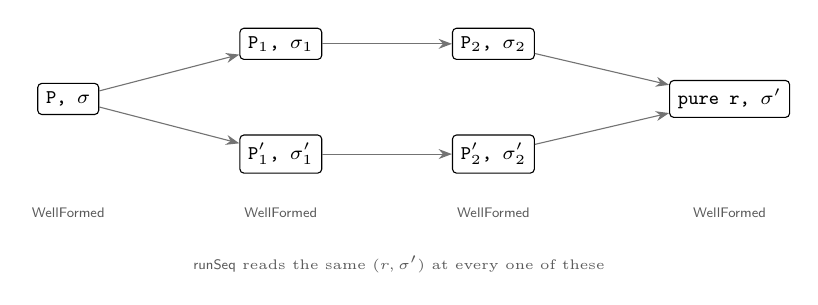
\begin{tikzpicture}[>=Stealth, font=\small,
  c/.style ={draw,rounded corners=1.5pt,inner sep=3pt,font=\scriptsize\ttfamily},
  e/.style ={draw,black!55,line width=0.4pt,->},
  g/.style ={font=\tiny,inner sep=1.5pt,text=black!65}]

\node[c] (c0) at (0,0)    {P, $\sigma$};
\node[c] (c1) at (2.7,0.7)  {P$_1$, $\sigma_1$};
\node[c] (c2) at (2.7,-0.7) {P$_1'$, $\sigma_1'$};
\node[c] (c3) at (5.4,0.7)  {P$_2$, $\sigma_2$};
\node[c] (c4) at (5.4,-0.7) {P$_2'$, $\sigma_2'$};
\node[c] (cf) at (8.4,0)    {pure r, $\sigma'$};

\draw[e] (c0) -- (c1); \draw[e] (c0) -- (c2);
\draw[e] (c1) -- (c3); \draw[e] (c2) -- (c4);
\draw[e] (c3) -- (cf); \draw[e] (c4) -- (cf);

\node[g] at (0,-1.45)   {$\wf$};
\node[g] at (2.7,-1.45) {$\wf$};
\node[g] at (5.4,-1.45) {$\wf$};
\node[g] at (8.4,-1.45) {$\wf$};
\node[g,align=center] at (4.2,-2.1)
  {$\runSeq$ reads the same $(r,\sigma')$ at every one of these};
\end{tikzpicture}
\caption{Lemma~\ref{lem:preserved} carries $\wf$ across one edge and
Lemma~\ref{lem:stepcombined} carries $\runSeq$'s value; Lemma~\ref{lem:chain} iterates both
along any path. Different paths may visit different configurations, but every path ends at
the one outcome $\runSeq$ named at the start.}\label{fig:invariant}
\end{figure}

\subsection{Safety: the forward direction}\label{sec:canonical:safe}

\begin{proof}[Proof of Theorem~\ref{thm:canonical}, direction $\Longrightarrow$]
Suppose $\wf\ p\ \st$ and
$\Reaches\ \langle p, \st\rangle\ \langle \texttt{pure}\ r, \st'\rangle$. Apply
Lemma~\ref{lem:chain} to that run, with $P' \coloneqq \texttt{pure}\ r$ and the memory
$\st'$. It gives
\[
  \runSeq\ (\texttt{pure}\ r)\ \st' = \runSeq\ p\ \st .
\]
By Definition~\ref{def:runseq}'s first line, $\runSeq\ (\texttt{pure}\ r)\ \st' = (r,\st')$.
Substituting, $(r,\st') = \runSeq\ p\ \st$, as required.
\end{proof}

Three lines. That is the payoff of finding the right invariant: once the conserved quantity is
known, safety is immediate. Note that this direction uses \emph{no induction on the program
at all} --- the induction happened inside Lemmas~\ref{lem:stepcombined}--\ref{lem:chain}.

\subsection{Liveness: the backward direction}\label{sec:canonical:live}

\begin{scratch}
We are asked to show something is \emph{reachable}, which calls for a construction: exhibit a
schedule. And we know which one to try --- the left-to-right one, because that is the one
$\runSeq$ describes. So the content of this direction is only: \emph{the sequential schedule
is a legal schedule}. The one thing that could go wrong is tripping the race test, and
Lemma~\ref{lem:norace} rules that out.
\end{scratch}

\begin{proof}[Proof of Theorem~\ref{thm:canonical}, direction $\Longleftarrow$]
By mutual induction on $p$, with the children-level motive $\mathit{motive}_2$ of
Theorem~\ref{thm:canonicalpair}.

\emph{Case $\texttt{pure}\ a$.} Here $\runSeq\ (\texttt{pure}\ a)\ \st = (a,\st)$, so $r = a$
and $\st' = \st$, and the required run is
$\Reaches\ \langle \texttt{pure}\ a, \st\rangle\ \langle \texttt{pure}\ a, \st\rangle$, which
is the $\mathsf{refl}$ rule.

\emph{Case $\texttt{read}\ l\ k$.} Since
$\runSeq\ (\texttt{read}\ l\ k)\ \st = \runSeq\ (k\,(\st\,l))\ \st$, we have
$(r,\st') = \runSeq\ (k\,(\st\,l))\ \st$; and since
$\wf\ (\texttt{read}\ l\ k)\ \st = \wf\ (k\,(\st\,l))\ \st$, the induction hypothesis applies
to $k\,(\st\,l)$ at $\st$ and gives
$\Reaches\ \langle k\,(\st\,l), \st\rangle\ \langle \texttt{pure}\ r, \st'\rangle$. Prepend
one step: $\langle k\,(\st\,l), \st\rangle \in \mathsf{step}\ (\texttt{read}\ l\ k)\ \st$ by
Definition~\ref{def:step}, so the $\mathsf{tail}$ rule and transitivity
(Proposition~\ref{prop:reachesbasic}) give the run from $\langle \texttt{read}\ l\ k, \st\rangle$.

\emph{Case $\texttt{write}\ l\ v\ k$.} Identical, at the memory $\upd{\st}{l}{v}$.

\emph{Case $\texttt{par}\ cs\ k$.} Write $(vs,\tau) = \mathsf{runChilds}\ cs\ \st$. Build the
schedule in five steps.
\begin{enumerate}[label=\arabic*.,leftmargin=2em,itemsep=1pt]
\item \emph{Run all the children to completion.} By $\mathit{motive}_2$, with hypotheses (W1)
      and (W2) from $\wf$, the children can collectively reach the configuration in which all
      are finished leaves holding $vs$, at memory $\tau$.
\item \emph{Check nothing races along the way.} By Lemma~\ref{lem:preserved} at the children
      level, $\mathsf{IndepAll}$ holds at every configuration of that run; by
      Lemma~\ref{lem:norace} it makes $\mathsf{racingAll}$ false at each one. So no
      configuration on this path goes to $\wrong$.
\item \emph{Lift it to the fork.} Lemma~\ref{lem:lift}(3) now applies, and gives
      \[
        \Reaches\ \langle \texttt{par}\ cs\ k,\ \st\rangle\
                  \langle \texttt{par}\ (\mathsf{pureChilds}\ vs)\ k,\ \tau\rangle .
      \]
\item \emph{Fire the join.} At that configuration every child is a $\texttt{pure}$ leaf, so
      every $\mathsf{nextAccs}$ is empty and $\mathsf{racingAll}$ is false; and
      $\mathsf{allPure}$ is $\mathsf{some}\ vs$. So Definition~\ref{def:step}'s second branch
      fires, with the single successor $\langle k\,vs, \tau\rangle$. That is one more step.
\item \emph{Finish in the continuation.} Conjunct (W3) is $\wf\ (k\,vs)\ \tau$, and by
      Definition~\ref{def:runseq}
      $\runSeq\ (\texttt{par}\ cs\ k)\ \st = \runSeq\ (k\,vs)\ \tau = (r,\st')$. So the
      continuation's induction hypothesis gives
      $\Reaches\ \langle k\,vs, \tau\rangle\ \langle \texttt{pure}\ r, \st'\rangle$.
\end{enumerate}
Compose steps 3, 4 and 5 by transitivity.

\emph{Children, empty spine.} $\mathsf{runChilds}\ [\,]\ \st = ((),\st)$ and the required run
is reflexivity.

\emph{Children, the $2$-to-$N$ step.} Write $(a,\tau_1) = \runSeq\ p\ \st$ and
$(ws,\tau_2) = \mathsf{runChilds}\ ps\ \tau_1$.
\begin{itemize}[leftmargin=1.6em,itemsep=1pt]
\item \emph{Run the head to completion}, applying the \emph{program-level} statement
      $\mathit{motive}_1$ to $p$ at $\st$. This is Theorem~\ref{thm:canonical} one level down,
      which is exactly why the two statements must be proved mutually. It gives
      $\Reaches\ \langle p, \st\rangle\ \langle \texttt{pure}\ a, \tau_1\rangle$.
\item \emph{Lift it}, tail standing still, by Lemma~\ref{lem:lift}(1).
\item \emph{Run the tail from there.} The tail's hypotheses hold at $\tau_1$, because that is
      how Definitions~\ref{def:childfootprints} and~\ref{def:wf} are stated --- each child
      measured from the memory the previous one left. The tail's induction hypothesis gives a
      collective run of $ps$ from $\tau_1$ to all-finished at $\tau_2$.
\item \emph{Lift it}, head standing still, by Lemma~\ref{lem:lift}(2).
\end{itemize}
Compose by transitivity. The result is $\texttt{pure}\ a$ followed by the finished tail at
$\tau_2$, which is $\mathsf{pureChilds}\ (a, ws)$ at $\tau_2$ --- and
$\mathsf{runChilds}\ (p :: ps)\ \st = ((a,ws),\tau_2)$ by Definition~\ref{def:runseq}.
\end{proof}

\begin{moral}
The liveness half contains no clever idea. It walks the left-to-right schedule and checks, at
each move, that the machine was \emph{allowed} to make it. That is all ``the sequential
schedule is one of the schedules'' means, and it is the half a soundness theorem omits.
\end{moral}

\subsection{Parallel equals sequential}\label{sec:canonical:parseq}

\begin{theorem}[Sequentialization]\label{thm:parseq}
If $\wf\ (\mathsf{parAll}\ ps)\ \st$ then
$\mathsf{parAll}\ ps \mathrel{\|\!\equiv} \mathsf{seqAll}\ ps$ from $\st$. In particular, if
$\wf\ (\mathsf{parPair}\ p\ q)\ \st$ then
$\mathsf{parPair}\ p\ q \mathrel{\|\!\equiv} \mathsf{seqPair}\ p\ q$ from $\st$.
\end{theorem}

\begin{scratch}
Theorem~\ref{thm:canonical} says each side has \emph{exactly one} possible outcome, named by
$\runSeq$. So to show the two sides have the same outcomes we need only show they have the
same $\runSeq$ value --- and that is pure unfolding, needing no independence at all.
\end{scratch}

\begin{proof}
We prove two claims and then apply Theorem~\ref{thm:canonical} to each side. Take the binary
case; the $N$-ary one is identical with a list in place of a pair. Write
$(a,\tau_1) = \runSeq\ p\ \st$ and $(b,\tau_2) = \runSeq\ q\ \tau_1$.

\begin{claim}\label{cl:samerunseq}
$\runSeq\ (\mathsf{parPair}\ p\ q)\ \st = \runSeq\ (\mathsf{seqPair}\ p\ q)\ \st$.
\end{claim}

\emph{The parallel side.} By Definition~\ref{def:combinators},
$\mathsf{parPair}\ p\ q = \texttt{par}\ \Pi[\,p\ q\,]\ (\lambda r.\ \texttt{pure}\ (r.1, r.2.1))$.
By Definition~\ref{def:runseq}'s children clause,
$\mathsf{runChilds}\ \Pi[\,p\ q\,]\ \st = ((a, (b, ())),\ \tau_2)$. So by the $\texttt{par}$
clause,
\[
  \runSeq\ (\mathsf{parPair}\ p\ q)\ \st = \runSeq\ (\texttt{pure}\ (a,b))\ \tau_2 = ((a,b),\ \tau_2) .
\]

\emph{The sequential side.} We need one fact about $\texttt{bind}$:
\begin{equation}
  \runSeq\ (\texttt{bind}\ x\ f)\ \st = \runSeq\ (f\,v)\ \tau, \qquad (v,\tau) = \runSeq\ x\ \st . \label{eq:runseqbind}
\end{equation}
\emph{Proof of~\eqref{eq:runseqbind}:} induction on $x$ using
Proposition~\ref{prop:induction}(i), which suffices because $\texttt{bind}$ leaves a fork's
children untouched. For $\texttt{pure}\ v$ we have $\texttt{bind}\ (\texttt{pure}\ v)\ f = f\,v$
and $\runSeq\ (\texttt{pure}\ v)\ \st = (v,\st)$, so both sides are $\runSeq\ (f\,v)\ \st$. For
$\texttt{read}\ l\ k$, $\texttt{bind}$ pushes inside, so the left side is
$\runSeq\ (\texttt{bind}\ (k\,(\st\,l))\ f)\ \st$ and the induction hypothesis applies.
$\texttt{write}$ and $\texttt{par}$ have the same shape.

Applying~\eqref{eq:runseqbind} twice to
$\mathsf{seqPair}\ p\ q = \texttt{bind}\ p\ (\lambda a.\ \texttt{bind}\ q\ (\lambda b.\ \texttt{pure}\ (a,b)))$:
\begin{align*}
  \runSeq\ (\mathsf{seqPair}\ p\ q)\ \st
  &= \runSeq\ (\texttt{bind}\ q\ (\lambda b.\ \texttt{pure}\ (a,b)))\ \tau_1 \\
  &= \runSeq\ (\texttt{pure}\ (a,b))\ \tau_2
   = ((a,b),\ \tau_2) .
\end{align*}
The two sides are equal, proving Claim~\ref{cl:samerunseq}. Note this is an equality of
$\runSeq$ \emph{values}, not merely of answers --- and note that \textbf{independence was
never mentioned}. It is a definitional identity between the reference run of a fork and the
reference run of a sequence, true even for racy programs, because $\runSeq$ is left-to-right
either way.

\begin{claim}\label{cl:seqwf}
$\wf\ (\mathsf{parPair}\ p\ q)\ \st$ implies $\wf\ (\mathsf{seqPair}\ p\ q)\ \st$.
\end{claim}

$\mathsf{seqPair}\ p\ q$ contains no $\texttt{par}$ node of its own, so
Definition~\ref{def:wf} imposes no independence obligation on it. Unfolding $\wf$ along
$\texttt{bind}$ --- an easy induction, companion to~\eqref{eq:runseqbind} ---
\[
  \wf\ (\texttt{bind}\ x\ f)\ \st \ \longleftrightarrow\ \wf\ x\ \st \wedge \wf\ (f\,v)\ \tau,
  \qquad (v,\tau) = \runSeq\ x\ \st ,
\]
and applying it twice reduces $\wf\ (\mathsf{seqPair}\ p\ q)\ \st$ to exactly
$\wf\ p\ \st$ and $\wf\ q\ \tau_1$. Both are conjunct (W2) of the hypothesis, which by
Definition~\ref{def:wf} unfolds to
$\wf\ p\ \st \wedge \wf\ q\ (\runSeq\ p\ \st).2 \wedge \mathtt{True}$. The memories match
because $\mathsf{runChilds}$ and $\texttt{bind}$ thread them in the same left-to-right order.
This proves Claim~\ref{cl:seqwf}.

\emph{Putting them together.} Fix any $r$ and $\st'$. Then
\begin{align*}
  &\Reaches\ \langle \mathsf{parPair}\ p\ q,\ \st\rangle\ \langle \texttt{pure}\ r,\ \st'\rangle \\
  &\quad \longleftrightarrow\ (r,\st') = \runSeq\ (\mathsf{parPair}\ p\ q)\ \st
      && \text{(Thm.~\ref{thm:canonical}, hypothesis)} \\
  &\quad \longleftrightarrow\ (r,\st') = \runSeq\ (\mathsf{seqPair}\ p\ q)\ \st
      && \text{(Claim~\ref{cl:samerunseq})} \\
  &\quad \longleftrightarrow\ \Reaches\ \langle \mathsf{seqPair}\ p\ q,\ \st\rangle\ \langle \texttt{pure}\ r,\ \st'\rangle
      && \text{(Thm.~\ref{thm:canonical}, Claim~\ref{cl:seqwf})}
\end{align*}
Since $r$ and $\st'$ were arbitrary, this is Definition~\ref{def:parseqeq}.
\end{proof}

\begin{remark}[Why the $N$-ary form is not a corollary of the binary one]
It is the other way round. $\mathsf{parAll}\ ps$ is a \emph{single} $\texttt{par}$ node with
all of $ps$ as children, so Claim~\ref{cl:samerunseq} holds for it by the same unfolding
(with an induction on $ps$ unfolding the nested $\mathsf{seqPair}$s), Claim~\ref{cl:seqwf} by
the same argument, and Theorem~\ref{thm:canonical} was already stated for arbitrary children
spines. There is no separate metatheory for $k$-way forks and no induction over a nest of
binary ones: a $k$-way fork is one node, and the induction over the children list happened
once, in Lemma~\ref{lem:stepcombined}'s $2$-to-$N$ step.
\end{remark}

\subsection{Strengthenings}\label{sec:canonical:strength}

Three refinements come free from the shape of the proof, and each is used in practice.

\begin{proposition}[Equal canonical runs suffice]\label{prop:runseqeq}
If $\wf\ p\ \st$, $\wf\ q\ \st$ and $\runSeq\ p\ \st = \runSeq\ q\ \st$, then
$p \mathrel{\|\!\equiv} q$ from $\st$.
\end{proposition}

\begin{proof}
Theorem~\ref{thm:canonical} on each side, exactly as in the final display above: both
reachability statements are equivalent to the same equation.
\end{proof}

This is the general form of Theorem~\ref{thm:parseq}: it is not about $\texttt{par}$ against
$\texttt{bind}$ at all, but about any two well-formed programs with the same reference run.
Theorem~\ref{thm:parseq} is the instance where Claim~\ref{cl:samerunseq} supplies the
hypothesis.

\begin{proposition}[Congruence]\label{prop:bindcongr}
Outcome equivalence is preserved by a prefix and by a continuation: if
$p \mathrel{\|\!\equiv} q$ from every memory reachable at that point, then
$\texttt{bind}\ r\ (\lambda\_.\ p) \mathrel{\|\!\equiv} \texttt{bind}\ r\ (\lambda\_.\ q)$, and
$\texttt{bind}\ p\ f \mathrel{\|\!\equiv} \texttt{bind}\ q\ f$.
\end{proposition}

\begin{proof}
Both reduce to Proposition~\ref{prop:runseqeq} via~\eqref{eq:runseqbind}: a $\texttt{bind}$'s
canonical run is determined by the prefix's canonical run and the continuation's, so equal
canonical runs on the pieces give equal canonical runs on the composite, and $\wf$ composes
the same way.
\end{proof}

Congruence is what lets a program with several parallel regions be sequentialised one region
at a time, rather than all at once.

\section{Cost: the same operations, fewer rounds}\label{sec:cost}

Theorem~\ref{thm:parseq} says the parallel program computes the same answer. It says nothing
whatever about speed, and a correct parallel program can easily be slower. So there is a
second thing to prove, and it has two halves that pull in opposite directions:
\begin{itemize}[leftmargin=1.6em,itemsep=1pt]
\item the total number of memory operations does \emph{not} go down --- parallelism reorders
      work, it does not delete it;
\item the number of \emph{rounds} does go down --- it becomes the maximum over the children
      instead of the sum.
\end{itemize}
The second is the interesting one, and the whole difficulty is to \emph{derive} the maximum
rather than to write it into a definition. A cost model that simply declared a fork's span to
be $\max$ of its children's spans would be assuming the result and proving nothing.

\subsection{Work}\label{sec:cost:work}

\begin{definition}[Work]\label{def:work}
$\work\ p\ \st$ counts the memory operations $p$ performs along its canonical run:
\begin{align*}
  \work\ (\texttt{pure}\ a)\ \st &= 0 \\
  \work\ (\texttt{read}\ l\ k)\ \st &= 1 + \work\ (k\,(\st\,l))\ \st \\
  \work\ (\texttt{write}\ l\ v\ k)\ \st &= 1 + \work\ (k\,())\ \upd{\st}{l}{v} \\
  \work\ (\texttt{par}\ cs\ k)\ \st &= \mathsf{workChilds}\ cs\ \st + \work\ (k\,vs)\ \tau,
    & (vs,\tau) = \mathsf{runChilds}\ cs\ \st \\
  \mathsf{workChilds}\ [\,]\ \st &= 0 \\
  \mathsf{workChilds}\ (p :: ps)\ \st &= \work\ p\ \st + \mathsf{workChilds}\ ps\ \tau_1,
    & (\_,\tau_1) = \runSeq\ p\ \st
\end{align*}
\end{definition}

Two features are worth noticing. A fork's work is the \emph{sum} over its children, not the
maximum: forking does not remove operations. And $\mathsf{workChilds}$ is staggered in exactly
the way $\mathsf{childFootprints}$ is (Definition~\ref{def:childfootprints}) --- each child
measured from the memory the previous one left --- because $\work$, like $\acc$, is measured
along the canonical run.

\begin{example}
For $p = \texttt{write}\ 5\ 1\ (\lambda\_.\ \texttt{pure}\ ())$ we get $\work\ p\ \st_0 = 1$,
and for $q = \texttt{read}\ 7\ (\lambda v.\ \texttt{write}\ 8\ v\ (\lambda\_.\ \texttt{pure}\ ()))$
we get $\work\ q\ \st = 2$ at every $\st$. So
$\work\ (\mathsf{parPair}\ p\ q)\ \st_0 = (1 + 2) + 0 = 3$: three operations, whether they are
run side by side or one after the other.
\end{example}

\begin{theorem}[Work is invariant]\label{thm:workeq}
$\work\ (\mathsf{parAll}\ ps)\ \st = \work\ (\mathsf{seqAll}\ ps)\ \st$, and in particular
$\work\ (\mathsf{parPair}\ p\ q)\ \st = \work\ (\mathsf{seqPair}\ p\ q)\ \st$. \textbf{No
independence hypothesis is needed.}
\end{theorem}

\begin{proof}
First, $\work$ adds across a $\texttt{bind}$:
\begin{equation}
  \work\ (\texttt{bind}\ x\ f)\ \st = \work\ x\ \st + \work\ (f\,v)\ \tau,
  \qquad (v,\tau) = \runSeq\ x\ \st . \label{eq:workbind}
\end{equation}
This is an induction on $x$ of the same shape as~\eqref{eq:runseqbind}: at
$\texttt{pure}\ v$ the left side is $\work\ (f\,v)\ \st$ and the right side is
$0 + \work\ (f\,v)\ \st$; at a $\texttt{read}$ or $\texttt{write}$ both sides gain the same
$1$ and the induction hypothesis closes the case; at a $\texttt{par}$ the children's summand
is untouched by $\texttt{bind}$ and the continuation's is the induction hypothesis.

Applying~\eqref{eq:workbind} along $\mathsf{seqAll}\ ps$ turns the right-hand side into the
staggered sum $\sum_i \work\ p_i\ \tau_i$, where $\tau_i$ is the memory left by the first $i$
children --- which is literally $\mathsf{workChilds}\ ps\ \st$ by
Definition~\ref{def:work}. And $\mathsf{parAll}\ ps$ is a single $\texttt{par}$ node with a
$\texttt{pure}$ continuation, so its work is $\mathsf{workChilds}\ ps\ \st + 0$. The two
agree.

The one thing to check is that the two sides measure their summands from the \emph{same}
memories, and they do, because by Claim~\ref{cl:samerunseq} the two sides have the same
canonical run, and $\mathsf{runChilds}$ and $\texttt{bind}$ thread memory in the same
left-to-right order.
\end{proof}

\begin{moral}
Work invariance needs no hypothesis at all, because $\work$ is a statement about the canonical
run --- and the canonical run of a fork \emph{is} the canonical run of the corresponding
sequence, racy or not. Everything that needs independence is about the \emph{real} runs.
\end{moral}

\subsection{Rounds: a second, derived relation}\label{sec:cost:rounds}

\begin{scratch}
We want to count how long a program takes on a machine with unlimited processors. The
semantics of Definition~\ref{def:step} will not do: it advances exactly \emph{one} child per
move, and its successor list \emph{branches}, so a path through it is a schedule and counting
its length counts a schedule's operations, not elapsed time.

So define a second relation in which one move advances \emph{every} child that is ready, all
at once, and which therefore has a \emph{single} successor and does not branch. Iterating a
non-branching relation is a count. Then prove the two relations agree --- that each of the new
relation's big moves is a legal sequence of the old relation's small moves. Without that
proof the round count would be a count of something imaginary.
\end{scratch}

\begin{definition}[Rounds]\label{def:pstep}
$\pstep\ p\ \st$ returns the residual program and the batch of writes the round performed, or
nothing if $p$ is finished:
\begin{align*}
  \pstep\ (\texttt{pure}\ a)\ \st &= \mathsf{none} \\
  \pstep\ (\texttt{read}\ l\ k)\ \st &= \mathsf{some}\ (k\,(\st\,l),\ [\,]) \\
  \pstep\ (\texttt{write}\ l\ v\ k)\ \st &= \mathsf{some}\ (k\,(),\ [(l,v)]) \\
  \pstep\ (\texttt{par}\ cs\ k)\ \st &=
    \begin{cases}
      \mathsf{some}\ (\texttt{par}\ cs'\ k,\ ws) & \pstep\mathsf{Childs}\ cs\ \st = \mathsf{some}\ (cs', ws) \\
      \pstep\ (k\,vs)\ \st & \text{otherwise, the join}
    \end{cases}
\end{align*}
where $\pstep\mathsf{Childs}$ advances \textbf{every} ready child in one round and concatenates
their write batches: a child that can move does, a child that cannot is left where it is, and
the round exists as long as at least one child moved.
\end{definition}

\begin{definition}[Applying a batch]\label{def:applyall}
$\mathsf{applyAll}\ \st\ ws$ performs a batch of writes on a memory, left to right:
\[
  \mathsf{applyAll}\ \st\ [\,] = \st, \qquad
  \mathsf{applyAll}\ \st\ ((l,v) :: ws) = \mathsf{applyAll}\ \upd{\st}{l}{v}\ ws .
\]
\end{definition}

The left-to-right order inside a batch looks like a choice that could matter, and in general it
does: if two children in the same round write the same cell, the last one wins and the answer
depends on the order of the spine. Under independence it cannot happen --- the children's write
sets are disjoint by clause (C1) of Definition~\ref{def:indep} --- so every address in the
batch is distinct and the order is immaterial. This is the first of several places where
independence quietly pays for the round model's right to exist.

\begin{remark}[Why there are two relations and not one]\label{rem:tworelations}
Figure~\ref{fig:roundvsstep} is the whole distinction. $\mathsf{stepChilds}$ returns one
successor \emph{per} ready child, so its successor list enumerates schedules; it is what
$\Reaches$ is built from, and what Theorem~\ref{thm:canonical} quantifies over.
$\pstep\mathsf{Childs}$ returns a \emph{single} successor in which every ready child has moved,
so iterating it counts rounds. The word $\max$ appears nowhere in
Definition~\ref{def:pstep}; it is derived in Theorem~\ref{thm:max}.
\end{remark}

\begin{figure}[htb]
\centering
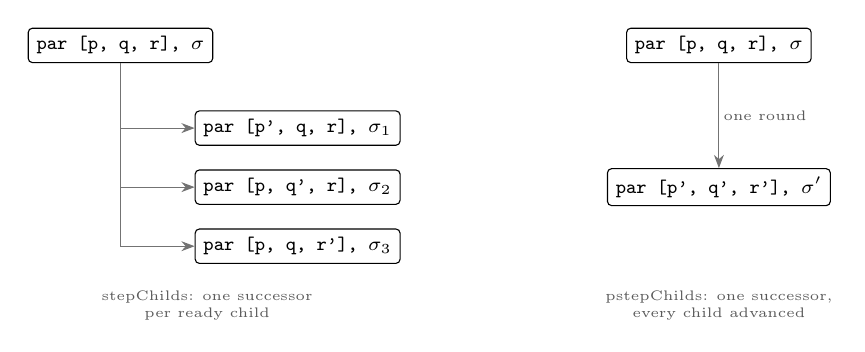
\begin{tikzpicture}[>=Stealth, font=\small,
  c/.style ={draw,rounded corners=1.5pt,inner sep=3pt,font=\scriptsize\ttfamily},
  e/.style ={draw,black!55,line width=0.4pt,->},
  g/.style ={font=\tiny,inner sep=1.5pt,text=black!65}]

\node[c] (a0) at (0,0) {par [p, q, r], $\sigma$};
\node[c] (a1) at (2.25,-1.05) {par [p', q, r], $\sigma_1$};
\node[c] (a2) at (2.25,-1.80) {par [p, q', r], $\sigma_2$};
\node[c] (a3) at (2.25,-2.55) {par [p, q, r'], $\sigma_3$};
\draw[e] (a0.south) |- (a1.west);
\draw[e] (a0.south) |- (a2.west);
\draw[e] (a0.south) |- (a3.west);
\node[g,align=center] at (1.1,-3.3) {stepChilds: one successor\\per ready child};

\node[c] (b0) at (7.6,0) {par [p, q, r], $\sigma$};
\node[c] (b1) at (7.6,-1.80) {par [p', q', r'], $\sigma'$};
\draw[e] (b0) -- node[g,right] {one round} (b1);
\node[g,align=center] at (7.6,-3.3) {pstepChilds: one successor,\\every child advanced};
\end{tikzpicture}
\caption{The same fork under the two relations. $\mathsf{stepChilds}$ branches, so a path
through it is a schedule; $\pstep\mathsf{Childs}$ does not branch, so iterating it is a count.
Lemma~\ref{lem:pstepreaches} is what ties the right-hand arrow back to a path on the
left.}\label{fig:roundvsstep}
\end{figure}

\begin{definition}[Span]\label{def:time}
$\mathsf{ptime}\ n\ p\ \st$ counts rounds under a fuel bound $n$: it returns $0$ when $n$ is
exhausted or when $\pstep$ is $\mathsf{none}$, and otherwise $1$ plus the count of the
residual at fuel $n-1$. The span is
\[
  \spn\ p\ \st \ \coloneqq\ \mathsf{ptime}\ (\work\ p\ \st + 1)\ p\ \st .
\]
\end{definition}

Why fuel, and not a termination argument? Because the recursion is on \emph{rounds}, and a
round is not a structurally smaller program --- a fork's round rebuilds a fork. Lean needs
some decreasing measure, and a counter is the honest one. The fuel never actually binds: a
round always performs at least one operation while the program is unfinished
(Lemma~\ref{lem:progress}), so $\work\ p\ \st$ rounds always suffice and the $+1$ is slack.

\subsection{A round is a legal sequence of ordinary steps}\label{sec:cost:realize}

\begin{lemma}[Realization]\label{lem:pstepreaches}
If $\wf\ p\ \st$ and $\pstep\ p\ \st = \mathsf{some}\ (p', ws)$ then
\[
  \Reaches\ \langle p, \st\rangle\ \langle p',\ \mathsf{applyAll}\ \st\ ws\rangle ;
\]
and if $\pstep\ p\ \st = \mathsf{none}$ then $p$ is already finished along its canonical run.
\end{lemma}

\begin{proof}
Mutual induction on $p$. A leaf's round is a single step, so the $\texttt{read}$,
$\texttt{write}$ and $\texttt{pure}$ cases are immediate, and the join case is one step of
Definition~\ref{def:step}'s second branch. Only the case of a fork with children moving has
content: a round in which $n$ children move \emph{at once} has to be exhibited as $n$
consecutive single-child moves, taken in spine order. Four things must hold for that sequence
to be a legal run.
\begin{enumerate}[label=(\arabic*),leftmargin=2em,itemsep=1pt]
\item \emph{Each move is available.} A child that $\pstep$ advances is, by
      Definition~\ref{def:pstep}, one that $\mathsf{step}$ can advance; so it appears in
      $\mathsf{stepChilds}$'s successor list at the moment its turn comes.
\item \emph{None of them trips the race test.} $\mathsf{IndepAll}$ holds at the start by
      hypothesis, and Lemma~\ref{lem:preserved} carries it across every move in the sequence,
      so Lemma~\ref{lem:norace} makes $\mathsf{racingAll}$ false at each one. Without this the
      sequence would reach $\wrong$ partway through and the run would not exist.
\item \emph{The memories match up at the end.} Performing the writes one child at a time, in
      spine order, must leave the same memory as $\mathsf{applyAll}$ applying the whole batch
      at once. The two agree because independence makes the children's write addresses
      distinct, so neither order can overwrite the other's cell --- fact (F1) of
      Definition~\ref{def:update} then gives equality cell by cell.
\item \emph{The spine is rebuilt correctly.} This is the $2$-to-$N$ step again: the head's
      moves are lifted to the spine by Lemma~\ref{lem:lift}(1) with the tail standing still,
      the tail's by Lemma~\ref{lem:lift}(2) with the head standing still, and the two compose
      by transitivity (Proposition~\ref{prop:reachesbasic}).
\end{enumerate}
\end{proof}

\begin{moral}
Lemma~\ref{lem:pstepreaches} is what makes the cost model honest. Without it, $\spn$ would be
the iteration count of a relation invented for the purpose, and a theorem about it would say
nothing about the programs. With it, every round is a real run of the real semantics, so
``$\spn\ p\ \st = 3$'' means a genuine three-batch execution exists.
\end{moral}

\begin{lemma}[A round preserves]\label{lem:pstepcombined}
Assume the hypotheses of Lemma~\ref{lem:pstepreaches}, and write
$\st_3 = \mathsf{applyAll}\ \st\ ws$. Then $\wf\ p'\ \st_3$, the canonical run is unchanged,
$\runSeq\ p'\ \st_3 = \runSeq\ p\ \st$, and the residual footprint is contained in the
original.
\end{lemma}

\begin{proof}
A round is a run, by Lemma~\ref{lem:pstepreaches}; and Lemma~\ref{lem:chain} establishes all
three statements along an arbitrary run. So there is nothing left to do: the conservation law
was already proved for paths, and a round is a path.
\end{proof}

\begin{lemma}[Non-interference of a round]\label{lem:pstepnonint}
If $\wf\ p\ \st$, the set $F$ is disjoint from $\acc\ p\ \st$, and $\st$ and $\st'$ agree
outside $F$, then $\pstep\ p\ \st = \pstep\ p\ \st'$. Consequently
$\mathsf{ptime}\ n\ p\ \st = \mathsf{ptime}\ n\ p\ \st'$ for every fuel $n$, and
$\spn\ p\ \st = \spn\ p\ \st'$.
\end{lemma}

\begin{proof}
The statement about one round is an induction mirroring Lemma~\ref{lem:locality}: at a
$\texttt{read}$ the address is outside $F$ so the two memories give the same value, at a
$\texttt{write}$ both sides write the same pair, and at a fork the case splits on which
children advance --- the same ones on both sides, by the children's induction hypothesis. At a
join every child is finished, so none has moved memory, and the continuation is entered at the
same program and the same memory on both sides.

The statement about the round \emph{count} is an induction on the fuel. After one round the
hypotheses must be re-established, and they are: well-formedness by
Lemma~\ref{lem:pstepcombined}, disjointness from $F$ by the footprint containment in the same
lemma, and the agreement of the two memories outside $F$ because applying one batch of writes
to two memories that agree outside $F$ leaves them agreeing outside $F$ --- every write in the
batch is at an address inside the footprint, hence outside $F$, and is the same write on both
sides.
\end{proof}

\begin{lemma}[A round makes progress]\label{lem:progress}
Under the hypotheses of Lemma~\ref{lem:pstepreaches},
\[
  \work\ p'\ (\mathsf{applyAll}\ \st\ ws) \ <\ \work\ p\ \st .
\]
Consequently $\mathsf{ptime}\ n\ p\ \st \le \work\ p\ \st$ for every $n$, the fuel never
binds, and $\mathsf{ptime}\ n\ p\ \st = \spn\ p\ \st$ for every $n > \work\ p\ \st$.
\end{lemma}

\begin{proof}
Mutual induction on $p$. For a $\texttt{read}$ or $\texttt{write}$, $\work$ drops by exactly
$1$ and the claim is immediate. The fork case is the one with content, and the reason is that
by Definition~\ref{def:work} a fork's work is a \emph{sum of two summands},
\[
  \work\ (\texttt{par}\ cs\ k)\ \st = \underbrace{\mathsf{workChilds}\ cs\ \st}_{\text{children}}
  \ +\ \underbrace{\work\ (k\,vs)\ \tau}_{\text{continuation}},
\]
and a round touches only the first. Each summand must be handled separately.

\emph{The children's summand strictly decreases.} At least one child moved --- that is what it
means for the round to exist --- and by the children's induction hypothesis that child's own
work strictly decreased. The children that did \emph{not} move are at the same program, but
not at the same memory: the movers' writes have changed the memory underneath them. So their
summands are not unchanged for free. They are unchanged by
Lemma~\ref{lem:pstepnonint}: a non-mover's footprint is disjoint from the movers' by
$\mathsf{IndepAll}$, and the new memory agrees with the old outside the movers' footprint, so
the non-mover's round count --- and with the same argument its $\work$ --- is the same at both.
Hence the children's sum strictly decreases.

\emph{The continuation's summand must cancel \emph{exactly}.} Here a bound is not enough.
Suppose we only knew that the continuation's work did not grow. Then the total could stay
exactly where it was --- children's sum down by $1$, continuation's up by $1$ --- and the
strict inequality would fail, taking the fuel argument down with it. What is needed is that
$k$ is applied to the \emph{same} results and started from the \emph{same} memory before and
after the round. And that is exactly what Lemma~\ref{lem:pstepcombined} supplies: equality of
canonical runs pins down both components of $\mathsf{runChilds}\ cs\ \st$ --- the tuple $vs$
passed to $k$, and the memory $\tau$ it starts from. So the continuation's summand is
\emph{literally the same number} on both sides, and cancels.

Given strict decrease, the three consequences follow by induction on the fuel: each round
spends at least one unit of work, so no more than $\work\ p\ \st$ rounds can occur, so any
fuel exceeding $\work\ p\ \st$ gives the same count.
\end{proof}

\subsection{\texorpdfstring{$\max$}{max} as a theorem}\label{sec:cost:max}

\begin{definition}[The children's span]\label{def:ptimechilds}
$\mathsf{ptimes}\ n\ cs\ \st$ is the list of the children's own round counts, each measured
from the \textbf{pre-fork} memory $\st$, and
\[
  \mathsf{ptimeChilds}\ n\ cs\ \st \ \coloneqq\ \mathsf{foldr}\ \max\ 0\ (\mathsf{ptimes}\ n\ cs\ \st) .
\]
\end{definition}

Nothing is staggered here, unlike $\mathsf{workChilds}$ and $\mathsf{childFootprints}$. That
is the point: the children run concurrently, so there is no ``memory the previous child left''
for a later child to start from. The staggered definitions were about the reference run; this
one is about elapsed time. And it is legitimate to measure every child from the same pre-fork
memory precisely because, under independence, it makes no difference which memory a child is
measured from --- Lemma~\ref{lem:pstepnonint}.

\begin{theorem}[The span law]\label{thm:max}
For every fuel $n$, every children spine $cs$, and every pure continuation,
\[
  \wf\ (\texttt{par}\ cs\ (\texttt{pure} \circ f))\ \st
  \ \longrightarrow\
  \mathsf{ptime}\ n\ (\texttt{par}\ cs\ (\texttt{pure} \circ f))\ \st
  = \mathsf{ptimeChilds}\ n\ cs\ \st .
\]
In particular, for two independent branches,
$\spn\ (\mathsf{parPair}\ p\ q)\ \st = \max\ (\spn\ p\ \st)\ (\spn\ q\ \st)$.
\end{theorem}

\begin{proof}
Induction on the fuel $n$.

\emph{Base and the finished case.} If $\pstep\mathsf{Childs}\ cs\ \st = \mathsf{none}$ then
every child is finished, so every entry of $\mathsf{ptimes}$ is $0$ and the fold is $0$; and
the fork takes the join branch into a $\texttt{pure}$ continuation, which has no round either.
Both sides are $0$. Likewise when the fuel is exhausted.

\emph{The step.} Otherwise $\pstep\mathsf{Childs}\ cs\ \st = \mathsf{some}\ (cs', ws)$, and by
Definition~\ref{def:pstep} the fork's round \emph{is} the children's round. So the left-hand
side is
\[
  1 + \mathsf{ptime}\ n\ (\texttt{par}\ cs'\ (\texttt{pure}\circ f))\ (\mathsf{applyAll}\ \st\ ws) ,
\]
and the induction hypothesis --- applicable because the residual fork is well-formed by
Lemma~\ref{lem:pstepcombined} --- rewrites this to
$1 + \mathsf{ptimeChilds}\ n\ cs'\ (\mathsf{applyAll}\ \st\ ws)$. What remains to prove is the
purely arithmetic statement
\begin{equation}
  \mathsf{ptimeChilds}\ (n{+}1)\ cs\ \st
  = 1 + \mathsf{ptimeChilds}\ n\ cs'\ (\mathsf{applyAll}\ \st\ ws), \label{eq:maxstep}
\end{equation}
and this is an induction over the spine. Take the children one at a time.
\begin{itemize}[leftmargin=1.6em,itemsep=1pt]
\item A child that \emph{moved} contributes $1 + (\text{its remaining rounds})$ on the left,
      and its remaining rounds on the right.
\item A child that did \emph{not} move is finished, contributing $0$ on both sides --- and its
      count is unaffected by the movers' writes, by Lemma~\ref{lem:pstepnonint}.
\end{itemize}
So~\eqref{eq:maxstep} reduces to two facts about $\max$ and the successor function:
\[
  \max\ (1+a)\ (1+b) = 1 + \max\ a\ b, \qquad \max\ (1+a)\ 0 = 1 + \max\ a\ 0 .
\]
Both are immediate, and together they let the $+1$ be pulled out of the fold. That is where
the maximum comes from: it is not asserted, it is what a fold of $\max$ does when every entry
either advances by one or is already zero.

Independence is spent exactly once in this proof, in the appeal to
Lemma~\ref{lem:pstepnonint}, to let each child's count be taken from the pre-fork memory.

\emph{The binary form} is the two-element case of the general law, since
$\mathsf{foldr}\ \max\ 0\ [a,b] = \max\ a\ (\max\ b\ 0) = \max\ a\ b$. There is no separate
binary argument.
\end{proof}

\begin{theorem}[Sequential composition adds]\label{thm:seqadd}
$\spn\ (\texttt{bind}\ p\ f)\ \st = \spn\ p\ \st + \spn\ (f\,a)\ \tau_1$ where
$(a,\tau_1) = \runSeq\ p\ \st$; in particular
$\spn\ (\mathsf{seqPair}\ p\ q)\ \st = \spn\ p\ \st + \spn\ q\ \tau_1$.
\end{theorem}

\begin{proof}
A round of a $\texttt{bind}$ is a round of the prefix until the prefix finishes, and a round of
the continuation thereafter; so the counts add. The induction is on the prefix, transporting
the fuel bound with Lemma~\ref{lem:progress}, which says any fuel above the work gives the
same count and so the two sides may be compared at a common bound.
\end{proof}

\begin{corollary}[Parallel is no slower]\label{cor:faster}
If $\wf\ (\mathsf{parPair}\ p\ q)\ \st$ then
$\spn\ (\mathsf{parPair}\ p\ q)\ \st \le \spn\ (\mathsf{seqPair}\ p\ q)\ \st$, with strict
inequality when both branches take at least one round. The same holds for $\mathsf{parAll}$
against $\mathsf{seqAll}$.
\end{corollary}

\begin{proof}
Theorem~\ref{thm:max} makes the left-hand side $\max\ a\ b$ and Theorem~\ref{thm:seqadd} makes
the right-hand side $a + b$, where $a = \spn\ p\ \st$ and $b = \spn\ q\ \tau_1$ --- the two
agreeing on where $b$ is measured by Lemma~\ref{lem:pstepnonint}. For natural numbers
$\max\ a\ b \le a + b$ always, and $\max\ a\ b < a + b$ as soon as both are positive. The
$N$-ary form is an induction on the list whose step is
$\max\ a\ (\mathsf{foldr}\ \max\ 0\ \mathit{rest}) \le a + \Sigma\ \mathit{rest}$.
\end{proof}

\begin{moral}
Theorems~\ref{thm:workeq} and~\ref{thm:max} together are the separation: the same operations,
fewer rounds. Notice which hypotheses each needs. Work invariance needs none, because it is a
statement about the canonical run. The span law needs $\wf$, and needs it essentially --- as
the next example shows, dropping it breaks the conclusion and not merely the proof.
\end{moral}

\begin{example}[The $\max$ law fails for interfering branches]\label{ex:racycost}
Take $p$ and $q$ both writing the same cell, say $p = \texttt{write}\ 5\ 1\ \cdots$ and
$q = \texttt{write}\ 5\ 2\ \cdots$. Definition~\ref{def:pstep} still assigns each a round count
of $1$, and still assigns their fork a round count of $1$: $\pstep$ has no race test, since it
was built to count and not to judge.

But in the real semantics the fork does not reach a terminal configuration in one round, or in
any number of rounds. By Definition~\ref{def:step} the first thing it does is consult
$\mathsf{racingAll}$, which is true --- both children's next writes are at cell $5$ --- so the
single successor is $\wrong$, which is absorbing.

So dropping $\wf$ from Theorem~\ref{thm:max} does not merely break the proof; the conclusion
becomes a count of rounds of an execution that does not exist. The hypothesis is what makes
Lemma~\ref{lem:pstepreaches} available, and Lemma~\ref{lem:pstepreaches} is what ties the
count to reality.
\end{example}

\section{The whole thing on one page}\label{sec:recap}

\subsection{Nine lines}\label{sec:recap:nine}

\begin{enumerate}[label=\arabic*.,leftmargin=2.2em,itemsep=2pt]
\item A memory is a function $\Loc \to \Val$, and updating one cell leaves the others alone.
      \hfill (Def.~\ref{def:update})
\item A program is a tree: leaves, reads, writes, and forks with $N$ children and a
      continuation. \hfill (Def.~\ref{def:parm})
\item $\runSeq$ runs that tree left to right. It is a total function, so it names \emph{one}
      answer. \hfill (Def.~\ref{def:runseq})
\item $\acc$ measures what a program touches along that run; a fork's children are measured
      staggered. \hfill (Defs.~\ref{def:acc}, \ref{def:childfootprints})
\item $\Indep$ is Bernstein: write--write, write--read and read--write disjoint. Shared reads
      are allowed. \hfill (Def.~\ref{def:indep})
\item $\wf$ asks for $\Indep$ at \emph{every} fork, measured along the canonical run.
      \hfill (Def.~\ref{def:wf})
\item A step advances one child, or joins, or --- if two children's next accesses collide ---
      goes to $\wrong$. \hfill (Def.~\ref{def:step})
\item $\runSeq$ is conserved by every step and $\wf$ survives every step, so along every path
      the one outcome $\runSeq$ named at the start is the only one that can be reached, and it
      is reached. \hfill (Thm.~\ref{thm:canonical})
\item A fork and the corresponding sequence have the same $\runSeq$, by unfolding. So they have
      the same outcomes. \hfill (Thm.~\ref{thm:parseq})
\end{enumerate}

\noindent
Lines 1--7 are definitions; line 8 is the theorem; line 9 is ten lines of unfolding. The one
step with real content inside line 8 is sub-case B of Lemma~\ref{lem:stepcombined}: a child
that is not the leftmost moves, so the machine's memory and $\runSeq$'s reference memory
disagree, and independence is what makes the disagreement invisible.

\subsection{What rests on what}\label{sec:recap:deps}

\begin{figure}[htb]
\centering
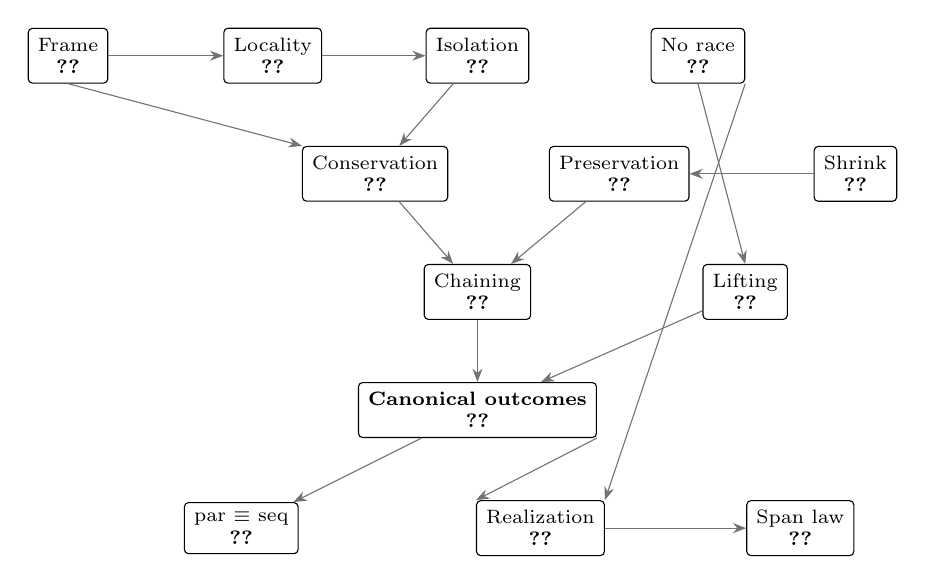
\begin{tikzpicture}[>=Stealth, font=\scriptsize,
  n/.style ={draw,rounded corners=1.5pt,inner sep=3.5pt,align=center,font=\scriptsize},
  e/.style ={draw,black!55,line width=0.4pt,->}]

\node[n] (frame)  at (0,0)      {Frame\\\ref{lem:frame}};
\node[n] (loc)    at (2.6,0)    {Locality\\\ref{lem:locality}};
\node[n] (iso)    at (5.2,0)    {Isolation\\\ref{lem:isolated}};
\node[n] (norace) at (8.0,0)    {No race\\\ref{lem:norace}};

\node[n] (cons)   at (3.9,-1.5) {Conservation\\\ref{lem:stepcombined}};
\node[n] (pres)   at (7.0,-1.5) {Preservation\\\ref{lem:preserved}};
\node[n] (shr)    at (10.0,-1.5){Shrink\\\ref{lem:subsetrw}};

\node[n] (chain)  at (5.2,-3.0) {Chaining\\\ref{lem:chain}};
\node[n] (lift)   at (8.6,-3.0) {Lifting\\\ref{lem:lift}};

\node[n] (canon)  at (5.2,-4.5) {\textbf{Canonical outcomes}\\\ref{thm:canonical}};

\node[n] (parseq) at (2.2,-6.0) {par $\equiv$ seq\\\ref{thm:parseq}};
\node[n] (real)   at (6.0,-6.0) {Realization\\\ref{lem:pstepreaches}};
\node[n] (span)   at (9.3,-6.0) {Span law\\\ref{thm:max}};

\draw[e] (frame) -- (loc);
\draw[e] (loc) -- (iso);
\draw[e] (iso) -- (cons);
\draw[e] (frame.south) -- (cons.north west);
\draw[e] (shr) -- (pres);
\draw[e] (cons) -- (chain);
\draw[e] (pres) -- (chain);
\draw[e] (chain) -- (canon);
\draw[e] (lift) -- (canon);
\draw[e] (norace.south) -- (lift.north);
\draw[e] (canon) -- (parseq);
\draw[e] (canon.south east) -- (real.north west);
\draw[e] (norace.south east) -- (real.north east);
\draw[e] (real) -- (span);
\end{tikzpicture}
\caption{The dependency structure. Frame through Preservation are statements about a
\emph{single} step; Chaining, Lifting and everything below them are statements about whole
runs. Independence enters at Isolation and No race, and nowhere else.}\label{fig:deps}
\end{figure}

\subsection{Where it breaks}\label{sec:recap:break}

A theorem whose hypothesis is never needed proves nothing. Two counterexamples show that
$\wf$ is load-bearing, and they fail in two \emph{different} ways --- which is why both are
needed.

\paragraph{Counterexample 1: the immediate race.}
Keep $p = \texttt{write}\ 5\ 1\ (\lambda\_.\ \texttt{pure}\ ())$ from
Example~\ref{ex:twoprogs} and replace $q$ by
\[
  q' = \texttt{read}\ 5\ (\lambda v.\ \texttt{write}\ 8\ v\ (\lambda\_.\ \texttt{pure}\ ())),
\]
which reads cell $5$ instead of cell $7$. Then
$\acc\ p\ \st_0 = (\varnothing, \{5\})$, while $\acc\ q'\ \tau = (\{5\}, \{8\})$ at
\emph{every} memory $\tau$, since $q'$ has no branches. So clause (C2) of
Definition~\ref{def:indep} fails:
$\writes{p} \cap \reads{q'} = \{5\} \neq \varnothing$. And indeed, at
$\texttt{par}\ \Pi[\,p\ q'\,]\ k$ the labels are $[\texttt{write}\ 5]$ and
$[\texttt{read}\ 5]$, which collide, so $\mathsf{racingAll}$ is true and
Definition~\ref{def:step} sends the configuration to $\wrong$ --- in \emph{one} step, before
anything else can happen. The program has \emph{no} terminating run at all, while
$\mathsf{seqPair}\ p\ q'$ has one. So Theorem~\ref{thm:canonical}'s $\Longleftarrow$ direction
fails here: the canonical outcome exists but is not reachable.

The repository's version of this failure is even blunter --- two branches that both write
cell $0$, one storing $1$ and one storing $2$ --- but the point is the same, and $p$ and $q'$
are already in hand.

This is the easy failure, and on its own it would leave a suspicion that $\wf$ is merely a
convenient way to say ``does not crash''.

\paragraph{Counterexample 2: the race that does not show up immediately.}
This is the one that matters, and the repository proves every part of it. Two cells,
$\mathit{shared} = 0$ and $\mathit{own} = 1$, and two programs:
\begin{align*}
  \mathit{observer} &= \texttt{write}\ \mathit{own}\ 7\ (\lambda\_.\ \texttt{read}\ \mathit{shared}\ \texttt{pure}) \\
  \mathit{mutator}  &= \texttt{write}\ \mathit{shared}\ 99\ \texttt{pure}
\end{align*}
The observer stamps its own private cell and then \emph{reports} what $\mathit{shared}$ holds;
the mutator overwrites $\mathit{shared}$. Start from $\st_0$, in which cell $0$ holds $1$ and
every other cell holds $0$, and consider
$\texttt{par}\ \Pi[\,\mathit{observer}\ \mathit{mutator}\,]\ k$.

\emph{The first step is race-free.} The labels are $[\texttt{write}\ \mathit{own}]$ and
$[\texttt{write}\ \mathit{shared}]$ --- cells $1$ and $0$, different cells. So
$\mathsf{racingAll}$ is \textbf{false} and the machine proceeds happily, which is the entire
point of this example.

\emph{Two of its schedules.}
\begin{itemize}[leftmargin=1.6em,itemsep=1pt]
\item \emph{Run the mutator to completion first.} Memory becomes cell $0 \mapsto 99$. Then the
      observer writes cell $1 \mapsto 7$ and reads cell $0$, getting $99$. The fork joins with
      the answer $(99, ())$. This schedule \textbf{terminates}.
\item \emph{Let the observer take its own write first.} Memory becomes cell $1 \mapsto 7$, and
      the fork is now $\texttt{read}\ \mathit{shared}$ against
      $\texttt{write}\ \mathit{shared}$ --- the same cell. $\mathsf{racingAll}$ is true, and
      the next step is $\wrong$.
\end{itemize}

\emph{The sequential program has one outcome, and it is not that one.} Along $\runSeq$ the
observer runs first and completely, so its read of $\mathit{shared}$ happens \emph{before} the
mutator's write and sees the starting value $1$. Hence
$\runSeq\ (\mathsf{seqPair}\ \mathit{observer}\ \mathit{mutator})\ \st_0$ has answer
$(1, ())$, and by Theorem~\ref{thm:canonical} --- which applies, because a $\texttt{bind}$
chain contains no fork and so is well-formed for free --- that is the \emph{only} outcome it
can reach.

So the parallel program reaches $(99,())$, the sequential program cannot, and
$\mathsf{parPair} \mathrel{\|\!\equiv} \mathsf{seqPair}$ is \textbf{false} at $\st_0$. The
hypothesis that fails is, as it must be, $\mathsf{IndepAll}$: the observer reads
$\{\mathit{shared}\}$ and the mutator writes $\{\mathit{shared}\}$, so clause (C3) of
Definition~\ref{def:indep} fails --- not at the first step, but one step further in.

\begin{moral}
Counterexample 2 is why the race test alone is not the hypothesis. Its first step is
\emph{race-free}, so no amount of checking the step in front of you can rule it out. The
hypothesis has to look at the whole footprint of each child, along its whole run, which is
exactly what Definitions~\ref{def:acc} and~\ref{def:childfootprints} do and why they are
stated the way they are.

The two counterexamples also break Theorem~\ref{thm:canonical} in two \emph{different} places.
Counterexample 1 kills the $\Longleftarrow$ direction: the canonical outcome is never reached,
because every schedule aborts at once. Counterexample 2 kills the $\Longrightarrow$ direction:
a schedule reaches an outcome that is \emph{not} the canonical one. A theorem proving only the
first would still hold of Counterexample 1, and would therefore be compatible with a parallel
program that simply never runs. That is the sense in which one-sided soundness is not enough,
promised back in \S\ref{sec:question}.
\end{moral}

\end{document}
